\vspace{-.5em}
\section{Results}
\label{exp}
We evaluate SVC first on a single node MySQL database to evaluate its accuracy, performance, and efficiency in a variety of materialized view 
scenarios.
We look at three main applications, join view maintenance, aggregate view maintenance, and a data cube application, on the standard TPCD benchmark 
and skewed version of the benchmark TPCD-Skew.
Then, we evaluate the outlier indexing approach in terms of improved query accuracy and also evaluate the overhead associated with using the index.
After evaluation on the benchmark, we present an end-to-end application of log analysis with a dataset from a video streaming company.
In this application, we look at the real query workload of the company and materialize views that could improve performance of these queries.
We implement SVC in Spark 1.1 and deploy it on a 10-node cluster to analyze 1TB of logs.

\subsection{Single-node Experimental Setup}
Our single node experiments are run on a r3.large Amazon EC2 node (2x Intel Xeon E5-2670, 15.25 GB Memory, and 32GB SSD Disk) with a MySQL version 5.6.15 database.
These experiments evaluate views from 10GB TPCD and TPCD-Skew datasets.
TPCD-Skew dataset \cite{tpcdskew} is based on the Transaction Processing Council's benchmark
schema but is modified so that it generates a dataset with values drawn from a Zipfian distribution instead of uniformly.
The Zipfian distribution \cite{mitzenmacher2004brief} is a long-tailed distribution with a single parameter $z=\{1,2,3,4\}$ which a larger
value means a more extreme tail.
$z=1$ corresponds to the basic TPCD benchmark. 
We implement incremental view maintenance with an ``update...on duplicate key insert" command.
We implement SVC's sampling operator with a linear hash written in C that is evoked in MySQL as a stored procedure.
In all of the applications, the updates are kept in memory in a temporary table, and we discount this loading time from our experiments.
We build an index on the primary keys of the view, the base data, but not on the updates.

Below we describe the view definitions and the queries on the views:

\textbf{Join View: } In the TPCD specification, two tables receive insertions and updates: \textbf{lineitem} and \textbf{orders}.
Out of 22 parameterized queries in the specification, 12 are group-by aggregates of the join of \textbf{lineitem} and \textbf{orders} (Q3, Q4, Q5, Q7, Q8, Q9, Q10, Q12, Q14, Q18, Q19, Q21).
Therefore, we define a materialized view of the foreign-key join of \textbf{lineitem} and \textbf{orders}, and compare incremental view maintenance and SVC.
We treat the 12 group-by aggregates as queries on the view.

\textbf{Aggregate View: } We apply SVC in an application similar to data cubes \cite{gray1997data}.
We define the following ``base cube" as a materialized view that calculates the total revenue 
grouped by distinct customer, nation, region, and part number.
The queries on this view are ``roll-up" queries that aggregate over 
subsets of the groups (e.g., total of all customers in North America).
The specification of this data cube and the queries are listed in the appendix \reminder{TR}.

\textbf{Complex Views:} We take the TPCD schema and denormalize the database, and treat each of the 22 
TPCD queries as views on this denormalized schema. 
The 22 TPCD queries are actually parameterized queries where parameters, such as the selectivity of the predicate, are randomly set by the TPCD \textsf{qgen} program.
Therefore, we use the program to generate 10 random instances of each query and use those as our materialized view.
We remove views with a small result set making them not suitable for sampling or are static.
10 out of the 22 sets of views can benefit from SVC, and the reasons why queries were excluded is listed in the appendix \reminder{TR}.

For each of the views, we generated \emph{queries on the views}.
Since the outer queries of our views were group by aggregates, we picked a random attribute $a$ from the group by clause and a random attribute $b$ from aggregation.
We use $a$ to generate a predicate.
For each attribute $a$, the domain is specified in the TPCD standard.
We select a random subset of this domain eg. if the attribute is country then the predicate can be \textsf{countryCode} > 50 and \textsf{countryCode} < 100.
We generated \sumfunc, \avgfunc, and \countfunc of the following form: 
\begin{lstlisting} [mathescape]
SELECT $f(b)$ FROM View 
WHERE subset of domain of a;
\end{lstlisting}
We generated 100 random aggregate queries for each view.

\subsection{Distributed Experimental Setup}
We evaluated performance on Apache Spark 1.1.0 with a 10 node r3.large Amazon EC2 cluster.
Systems like Spark are increasingly popular, and Spark supports materialization through a distributed data structure called an RDD \cite{zaharia2012resilient}.
In the most recent release of Spark, there is a SQL interface that allows users to persist query results in memory.

However, in real-world application, RDDs have limitations.
As RDDs are an immutable data structure, any maintenance must be done synchronously.
As Spark also does not have support for indices, we rely on partitioned joins for incremental maintenance of the views.
We partitioned the views by primary-by key, and apply a full outer join of the updates with the partitioned view.
With this set of experiments, we show that SVC implemented on Spark can help overcome some of these limitations and allow users to take advantage of materialized views and incremental maintenance.

We evaluate SVC on a 1TB dataset of logs from a video streaming company, Conviva \cite{conviva}.
The 1TB dataset is a denormalized user activity log corresponding to video views and various metrics such as data transfer rates, and latencies.
%1TB corresponded to a sample of customer data from 1 year of logs. \reminder{[privacy]}
With this dataset, there was a corresponding dataset of analyst SQL queries on the log table.
In this workload, there were annotated summary statistics queries, and we filtered for the most common types.
While, we cannot give the details of the queries, we can present some of the high-level characteristics of 8 summary-statistics type views. 
\begin{itemize} 
\item \textbf{V1.} Counts of various error types grouped by resources, users, date
\item \textbf{V2.} Sum of bytes transferred grouped by resource, users, date
\item \textbf{V3.} Counts of visits grouped by an expression of resource tags, users, date.
\item \textbf{V4.} Nested query that groups users from similar regions/service providers together then aggregates statistics
\item \textbf{V5.} Nested query that groups users from similar regions/service providers together then aggregates error types
\item \textbf{V6.} Union query that is filtered on a subset of resources and aggregates visits and bytes transferred
\item \textbf{V7.} Aggregate network statistics group by resources, users, date with many aggregates.
\item \textbf{V8.} Aggregate visit statistics group by resources, users, date with many aggregates.
\end{itemize}
We used this dataset to evaluate the end-to-end accuracy and performance of the system in a real-world application.

Using the dataset of analyst queries, we identified 8 common summary statistics-type queries that calculated engagement and error-diagnosis metrics for specific customers on a certain day.
We generalized these queries by turning them into group-by queries over customers and dates; that is a view that calculates the metric for every customer on every day.
We generated aggregate random queries over this dataset by taking either random time ranges or random subsets of customers.

\subsubsection{Metrics and Evaluation}
To illustrate how SVC gives the user access to this new trade-off space, we will illustrate that SVC is more accurate than the stale query result (No Maintenance); but is less computationally intensive than full IVM. 

In our evaluation, we separate maintenance from query processing.
We use the following notation to represent the different approaches:
\begin{itemize}
\item No maintenance (Stale): The baseline for evaluation is not applying any maintenance to the materialized view.
\item Incremental View Maintenance (IVM): We apply incremental view maintenance to the full view.
\item SVC+AQP: We maintain a sample of the materialized view using SVC but estimate the result with AQP rather than using 
the correction technique proposed in this paper.
\item SVC+Corr: We maintain a sample of the materialized view using SVC and process queries on the view using the correction method presented in this paper.
\end{itemize}
%\reminder{Do you think we need to say something about another solution which maintains a sample of ``base" table and transform a query on a view to a query on the base table?}
Since SVC has a sampling parameter, we denote a sample size of $x \% $ as SVC+Corr-x or SVC+AQP-x, respectively. 

To evaluate accuracy and performance, we define the following metrics:
\begin{itemize}
\item Relative Error: For a query result $r$ and an incorrect result $r'$, the relative error is \[\frac{\mid r-r' \mid}{r}.\] 
When a query has multiple results (a group-by query), then, unless otherwise noted, relative error is defined as the median over all the errors.
\item Maintenance Time: We define the maintenance time as the time needed to produce the up-to-date view for incremental view maintenance, and the time needed to produce the up-to-date sample in SVC. 
\end{itemize}

\subsection{Single-node Accuracy and Performance}

\subsubsection{Join View}

\begin{figure}[t]
\centering
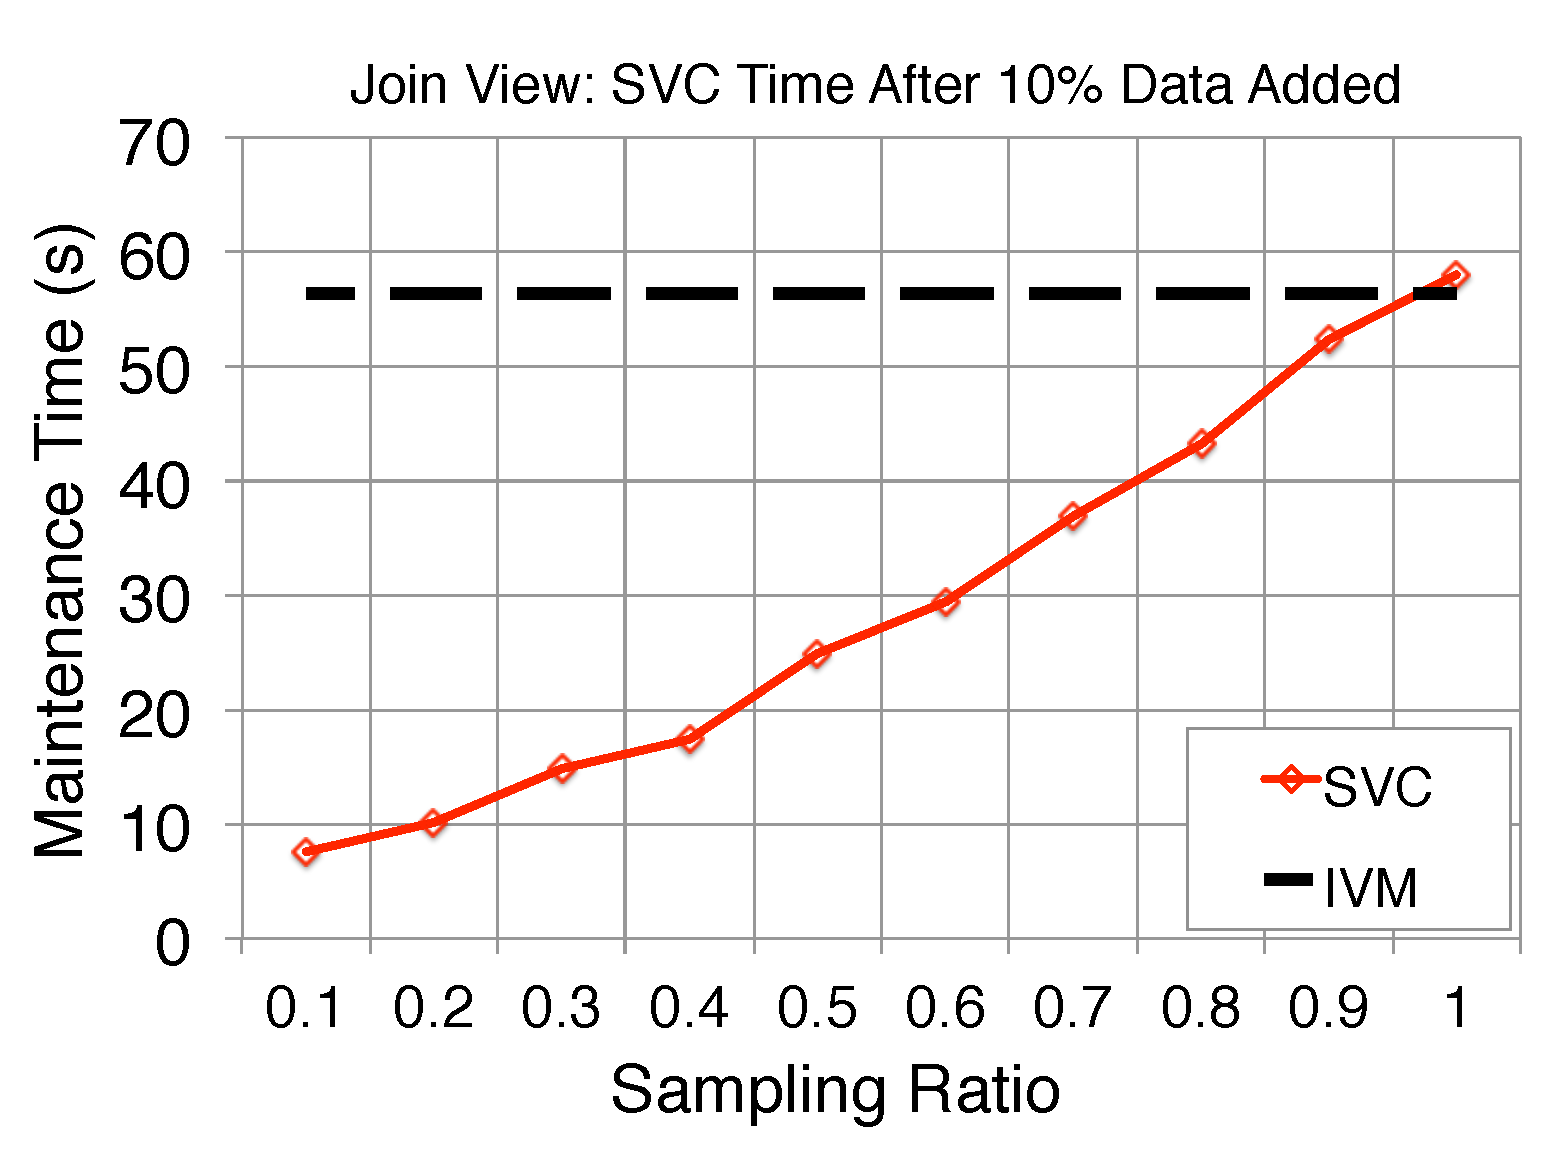
\includegraphics[scale=0.15]{exp/msj_1.pdf}
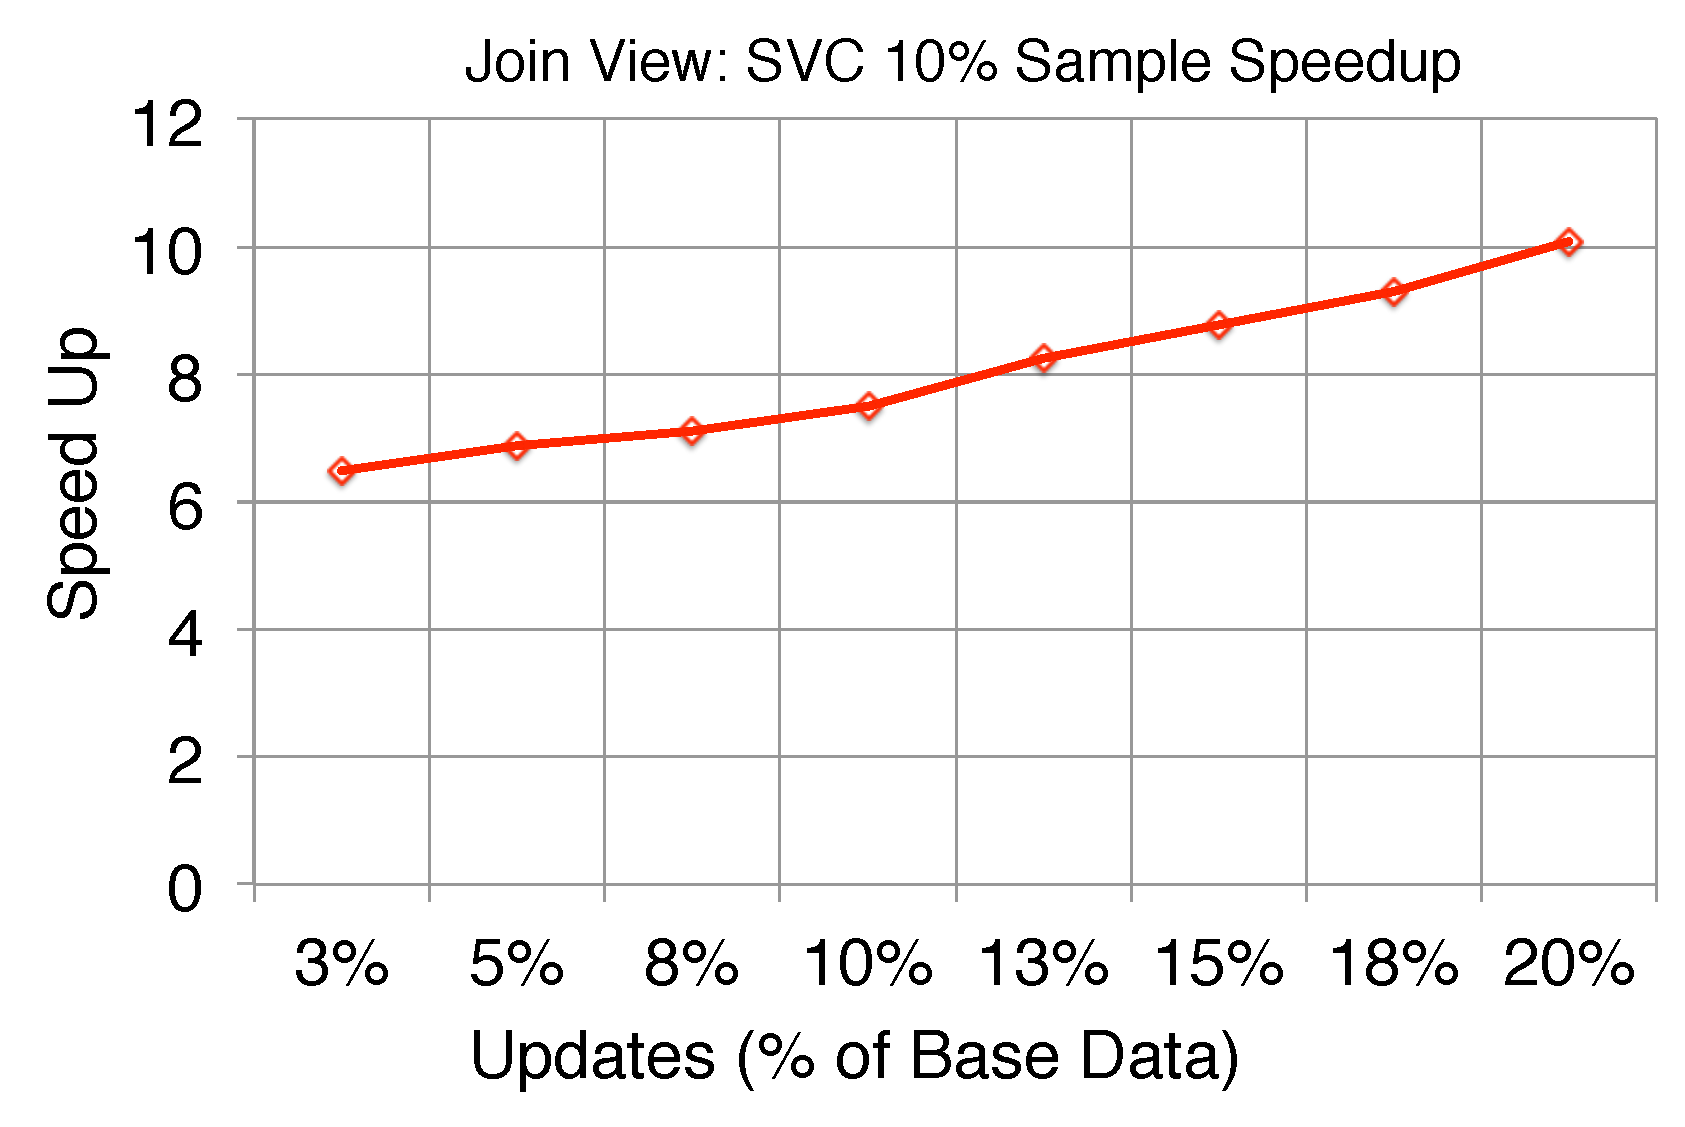
\includegraphics[scale=0.15]{exp/msj_2.pdf}
 \caption{(a) On a 10GB dataset with 1GB of insertions and updates, we vary the sampling ratio and measure the maintenance time of SVC. The black line marks the time for full incremental view maintenance. (b) For a fixed sampling ratio of 10\%, we vary the update size and plot the speedup compared to full incremental maintenance for SVC. \label{exp-1-samplesize}}
\end{figure}

\begin{figure}[t]
\centering
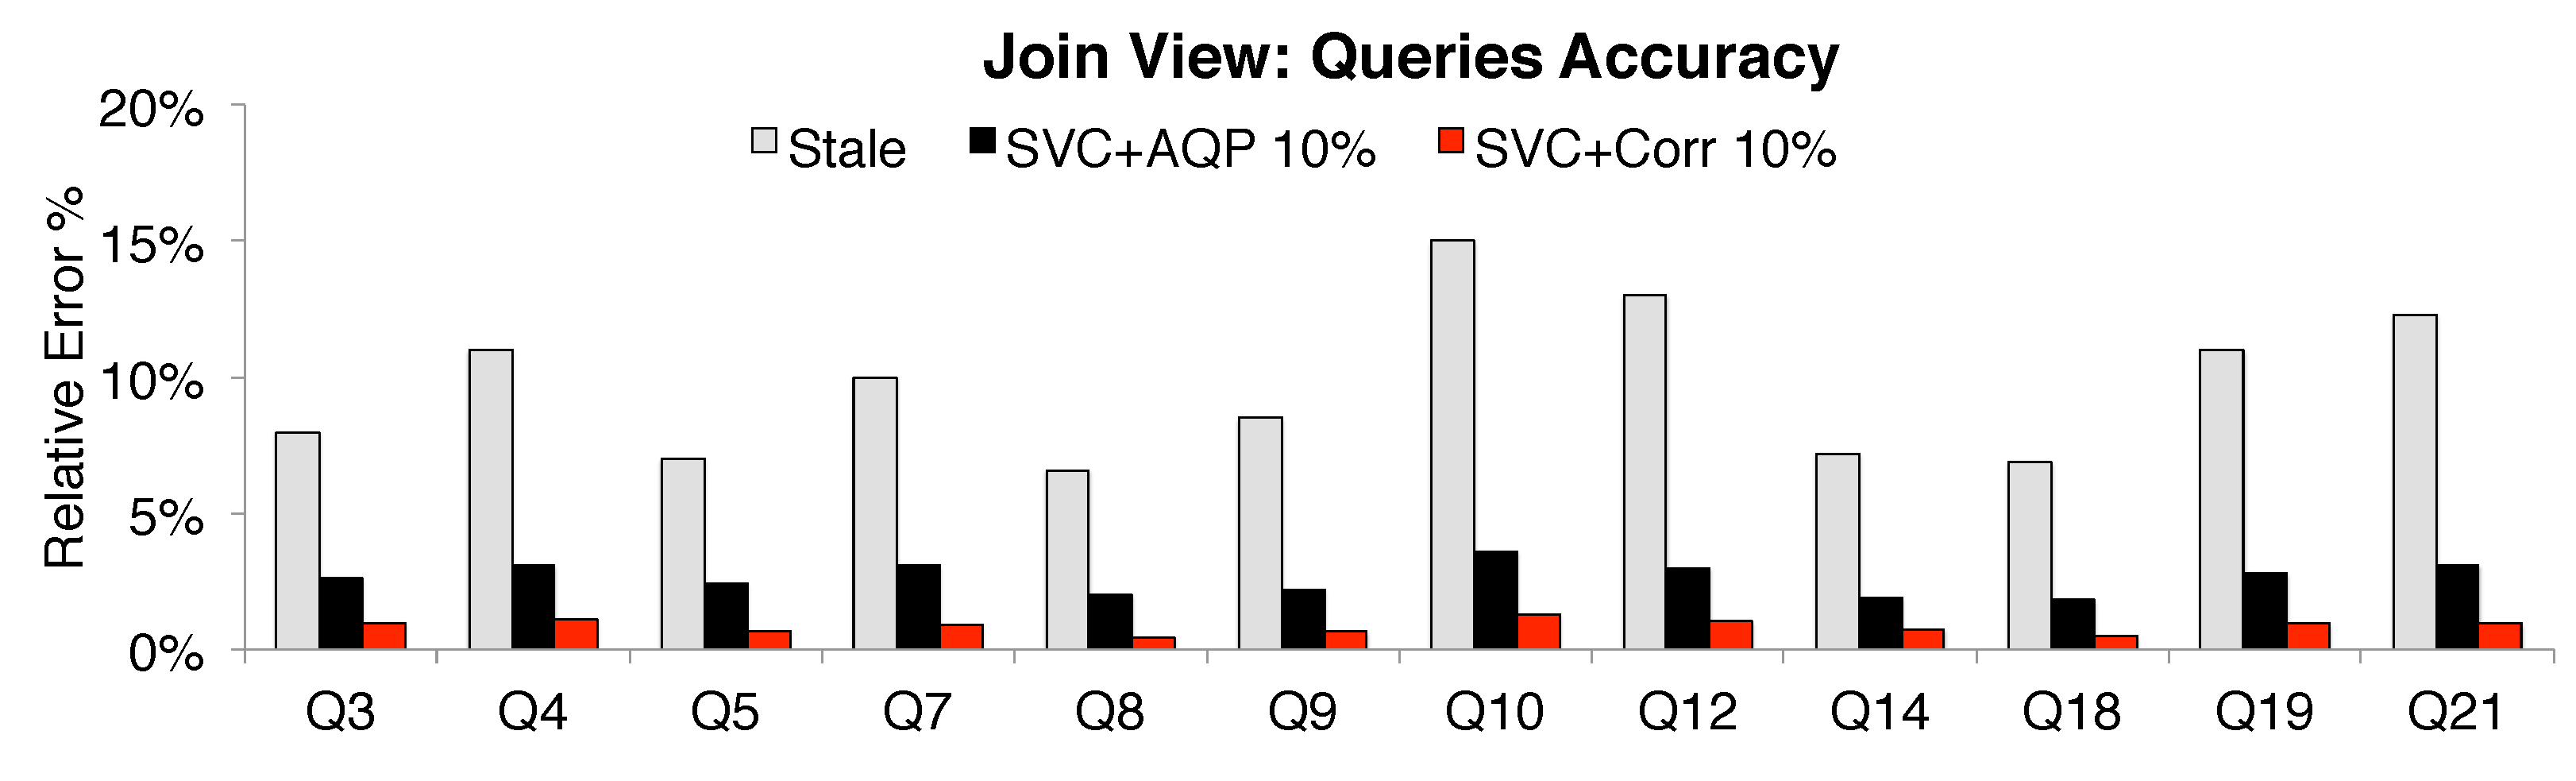
\includegraphics[scale=0.16]{exp/msj_3.pdf}
 \caption{We generate 100 of each TPCD parameterized query and answer it using the stale materialized view, SVC+Corr, and SVC+AQP. We plot the median relative error for each query (since the result for each query might be multi-valued). Our experiments suggest that on this view, SVC+Corr is more accurate than SVC+AQP and No Maintenance.\label{exp-1-acc}}
\end{figure}

\begin{figure}[t]
\centering
 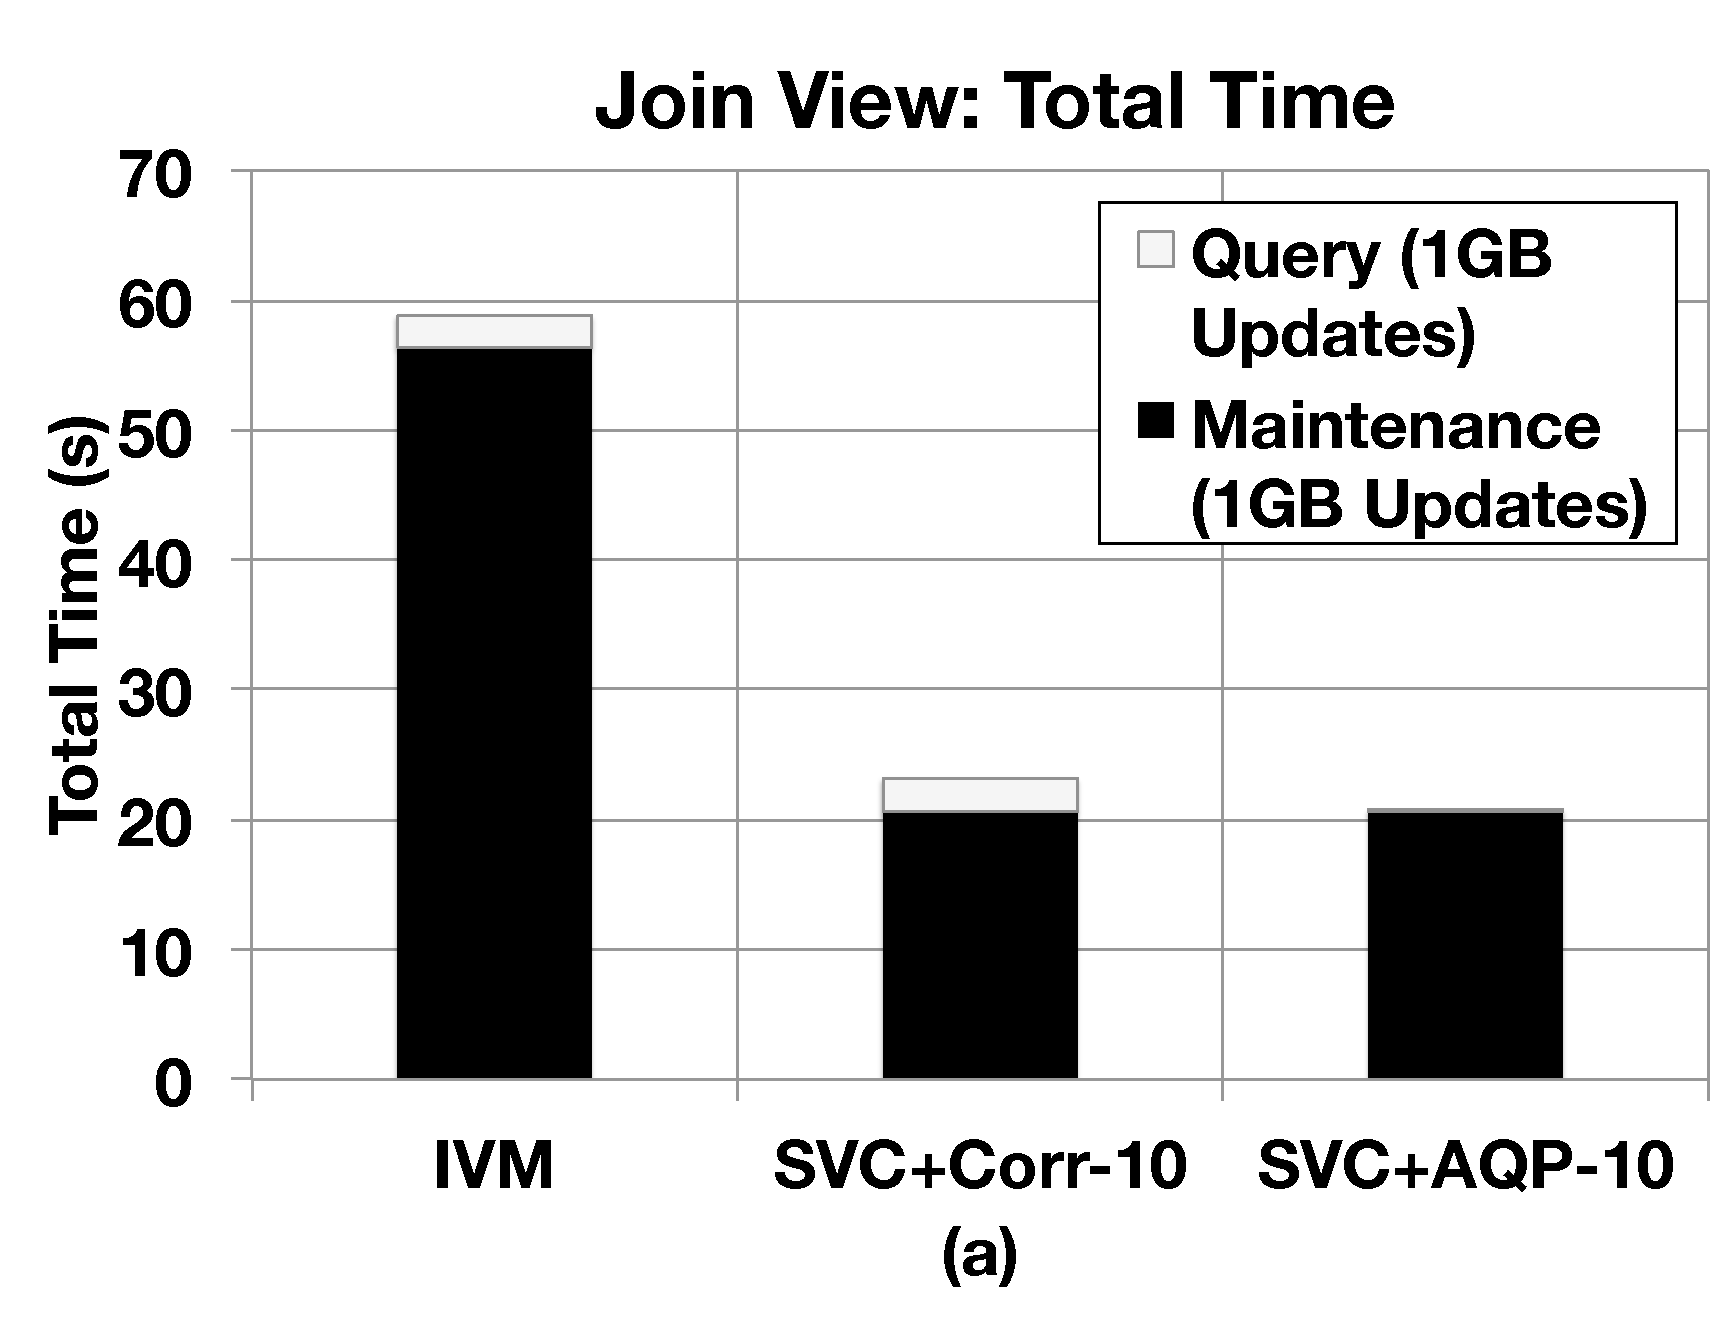
\includegraphics[scale=0.13]{exp/msj_4.pdf}
 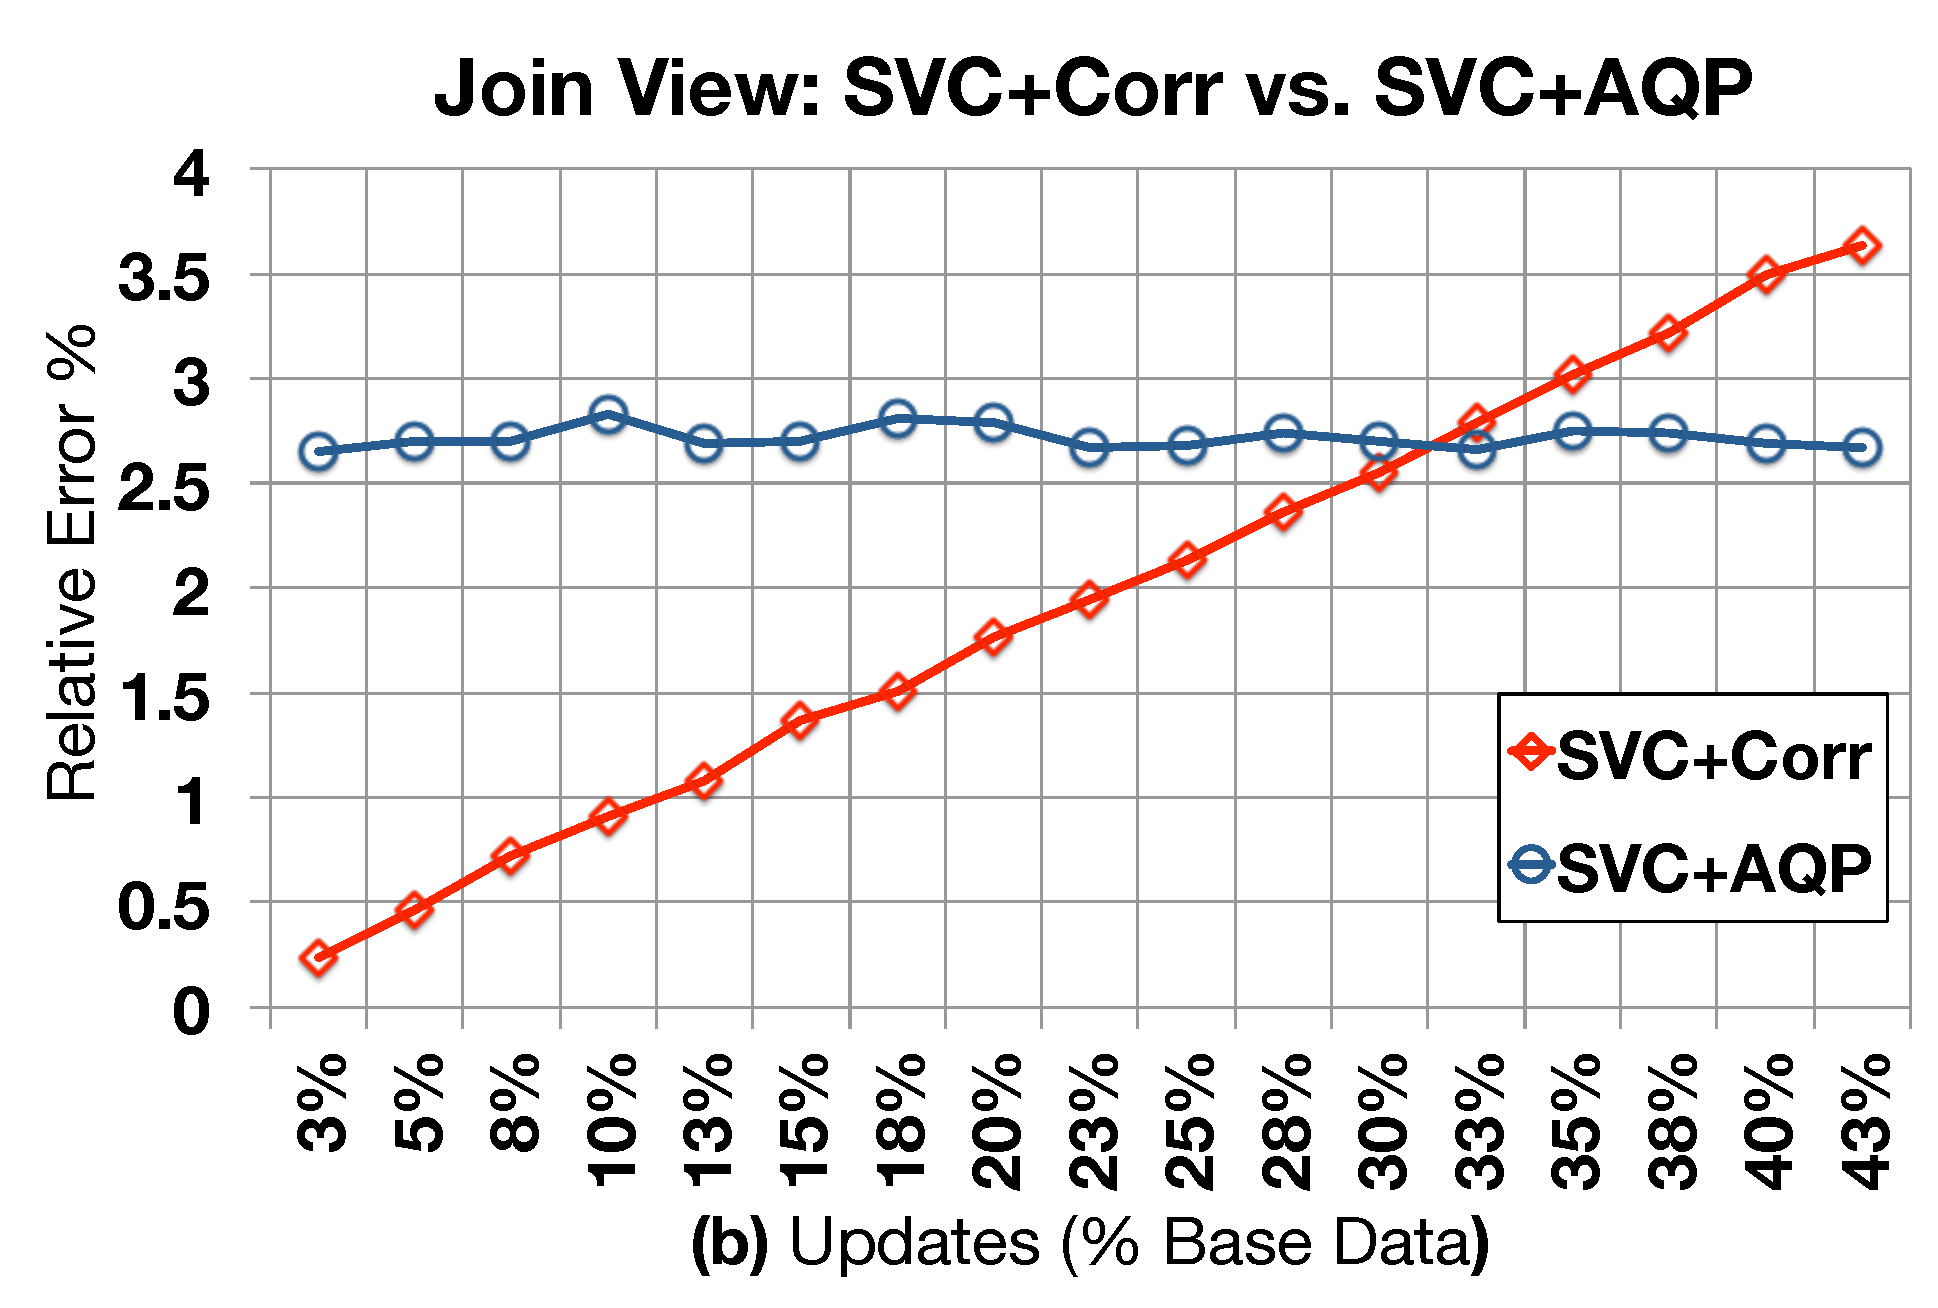
\includegraphics[scale=0.13]{exp/msj_6.pdf}
  \caption{(a) For a fixed sampling ratio of 10\% and update size of 10\% (1GB), we measure the total time incremental maintenance + query time. SVC+Corr does take longer to query a view (due to the correction) than SVC+AQP and IVM, but this overhead is small relative to to the savings in maintenance time. (b) We vary the update rate to show that SVC+Corr is more accurate than SVC+AQP until the update size is 32.5\% (3.2GB).  \label{exp-1-total}}
\end{figure}

\begin{figure}[t]
\centering
  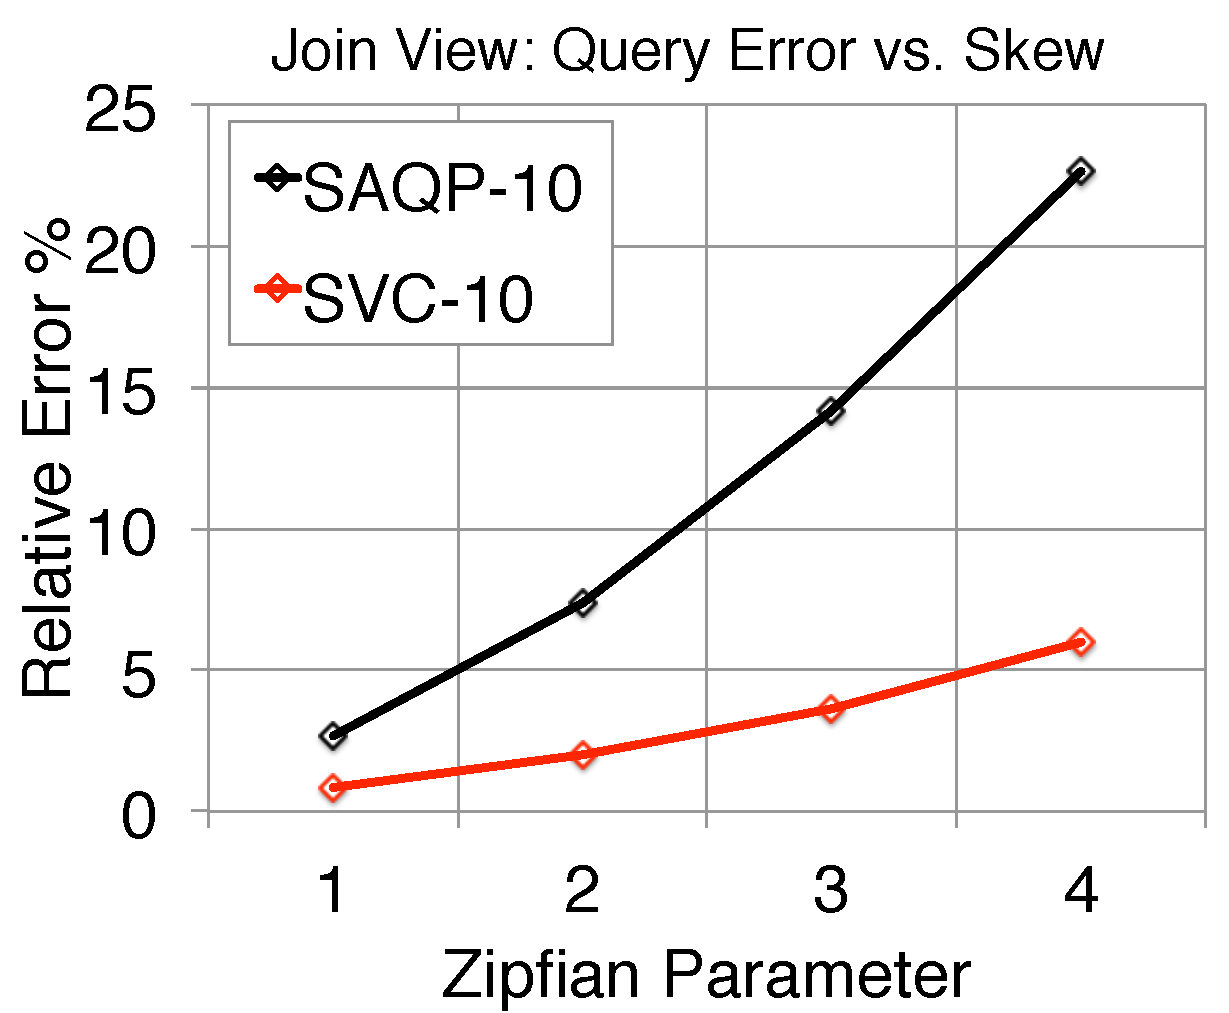
\includegraphics[scale=0.25]{exp/msj_5.pdf}
 \caption{We fix the update size at 1GB and the sampling ratio at 10\% and vary the skew of the dataset. The gap between SVC+AQP and SVC increases in more skew datasets suggesting that corrections are more robust to skew. \label{exp-1-zipf}}
\end{figure}

In our first experiment, we evaluate how SVC performs on a materialized view of the join of \textbf{lineitem} and \textbf{orders}.
We generate a 10GB base TPCD dataset with skew $z=1$, and derive the view from this dataset.
We first generate 1GB (10\% of the base data) of updates (insertions and updates to existing records), and vary the sample size.
Figure \ref{exp-1-samplesize}(a), shows the maintenance time of SVC as a function of sample size.
With the bolded dashed line, we note the time for full IVM. 
For this materialized view, sampling allows for significant savings in maintenance time; albeit for approximate answers.
While full incremental maintenance takes 56 seconds, SVC with a 10\% sample can complete in 7.5 seconds.

\textbf{Performance: }
The speedup for SVC-10 is 7.5x which is far from ideal on a 10\% sample.
In the next figure, Figure \ref{exp-1-samplesize}b, we evaluate this speedup. 
We fix the sample size to 10\% and plot the speedup of SVC compared to IVM while varying the size of the updates.
On the x-axis is the update size as a percentage of the base data.
For small update sizes, the speedup is smaller, 6.5x for a 2.5\% (250GB) update size.
As the update size gets larger, SVC becomes more efficient, since for a 20\% update size (2GB), the speedup is 10.1x. 
The super-linearity is because this view is a join of \textbf{lineitem} and \textbf{orders} and we assume that there is not a join index on the updates.
Since both tables are growing sampling reduces computation super-linearly. 

\textbf{Accuracy: }
At the same design point with a 10\% sample, we evaluate the accuracy of SVC.
In Figure \ref{exp-1-acc}, we answer TPCD queries with this view.
The TPCD queries are group-by aggregates and we plot the median relative error for SVC+Corr, No Maintenance, and SVC+AQP.
On average over all the queries, we found that SVC was 11.7x more accurate than the stale baseline, and 3.1x more accurate than applying SVC+Corr to the sample.

\textbf{SVC+Corr vs. SVC+AQP: }
While more accurate, it is true that SVC+Corr correction technique moves some of the computation from maintenance to query execution.
SVC+Corr calculates a correction to a query on the full materialized view.
On top of the query time on the full view (as in IVM) there is additional time to calculate a correction from a sample.
On the other hand SVC+AQP runs a query only on the sample of the view, 
Accordingly, for a 10\% sample SVC+Corr required 2.69 secs to execute a \sumfunc over the whole view, IVM required 2.45 secs, and  SVC+AQP required 0.25 secs.
However, when we compare this overhead to the savings in maintenance time it is small.
We evaluate this overhead in Figure \ref{exp-1-total}a, where we compare the total time maintenance and query execution time.

SVC+Corr is most accurate when the materialized view is less stale, since it relies on correct a stale result.
On the other hand SVC+AQP is more robust to the staleness and gives a consistent relative error.
The error for SVC+Corr grows proportional to the staleness.
In Figure \ref{exp-1-total}b, we explore which query processing technique should be used SVC+Corr or SVC+AQP.
For a 10\% sample, we find that SVC+Corr is more accurate until the update size is 32.5\% of the base data.

\textbf{Effect of Skew: }
Finally in Figure \ref{exp-1-zipf}, we vary the Zipfian parameter and show how the accuracy of SVC+Corr and SVC+AQP changes.
While both techniques are sensitive to skew, we find that the gap between SVC+Corr and SVC+AQP widens for more skewed datasets. 
SVC's accuracy is dependent on the variance of the difference between tuples in the up-to-date view and the stale view; which is different from SVC+AQP which is dependent on the variance of the tuples themselves. 
Even though a dataset might be skewed, if (in relative terms) the updates are more uniform SVC+Corr will give more accurate results.
We can make SVC+Corr and SVC+AQP even more accurate using the outlier indexing which we will evaluate in the later sections.

\subsubsection{Aggregate View}
\label{exp-datacube}

\begin{figure}[t]
\centering
 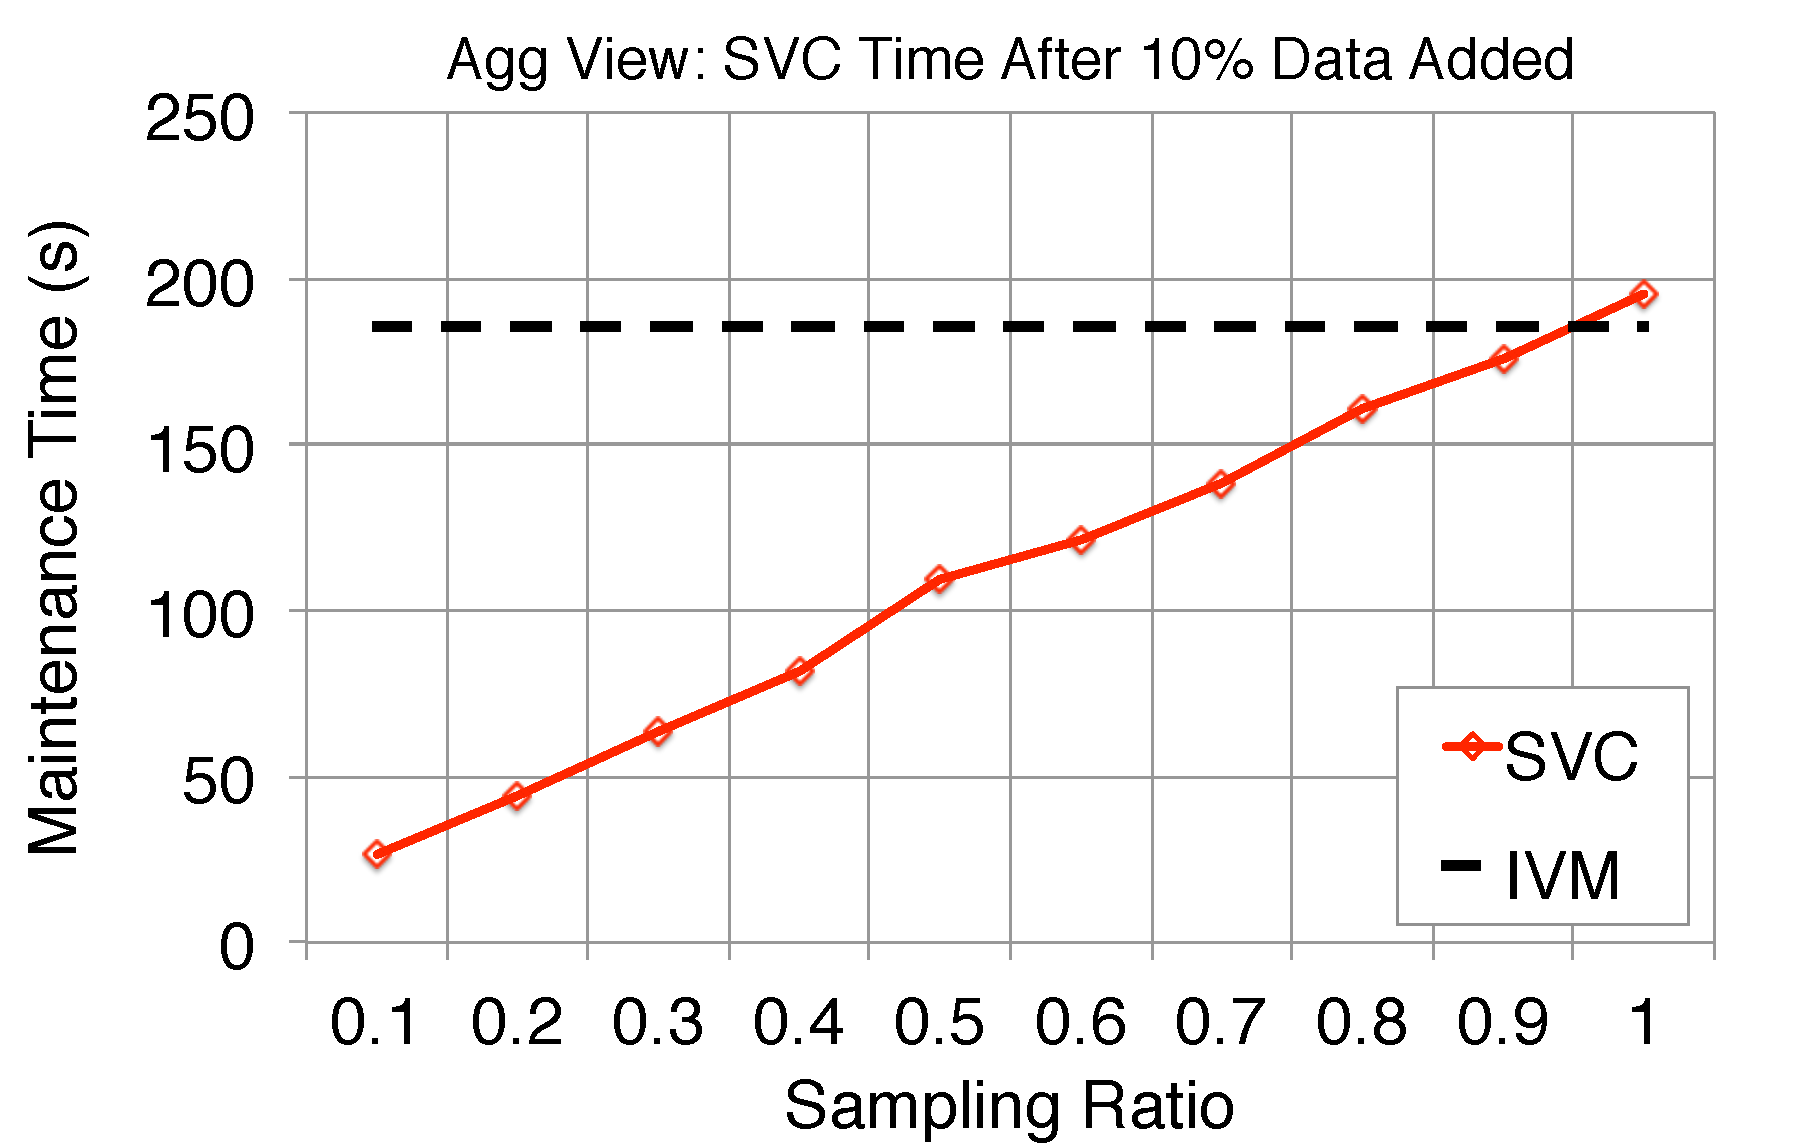
\includegraphics[scale=0.15]{exp/msdc_1.pdf}
 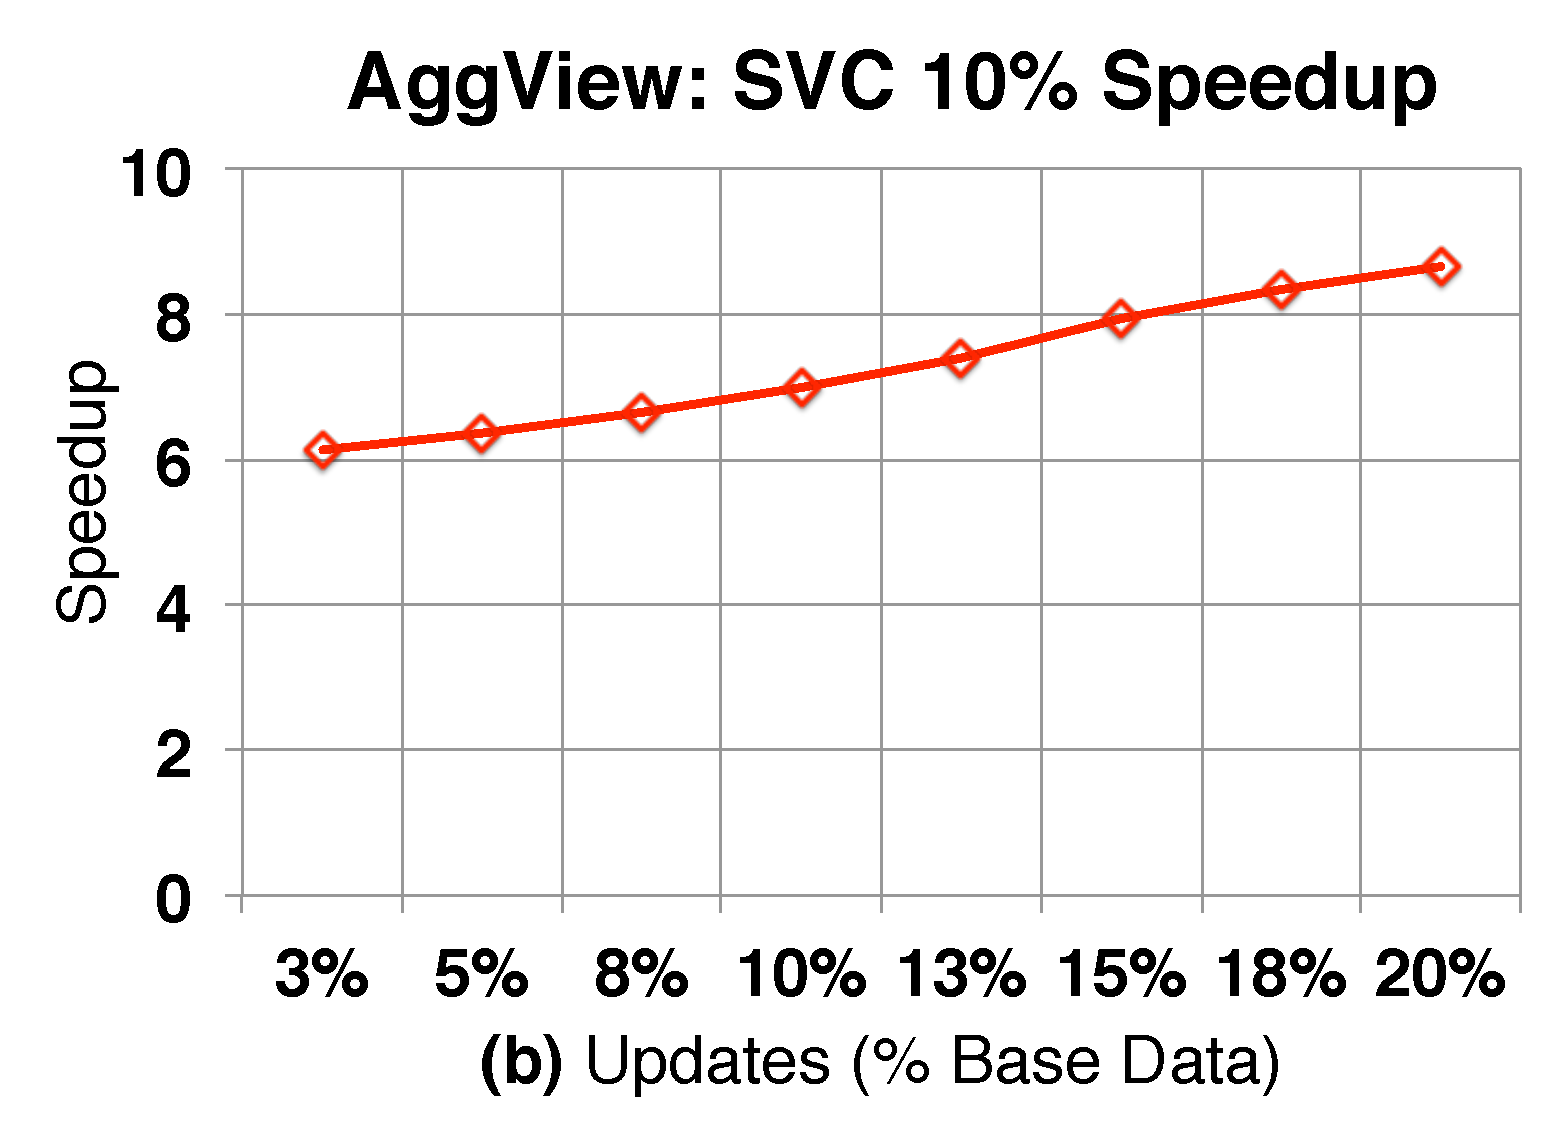
\includegraphics[scale=0.15]{exp/msdc_2.pdf}
  %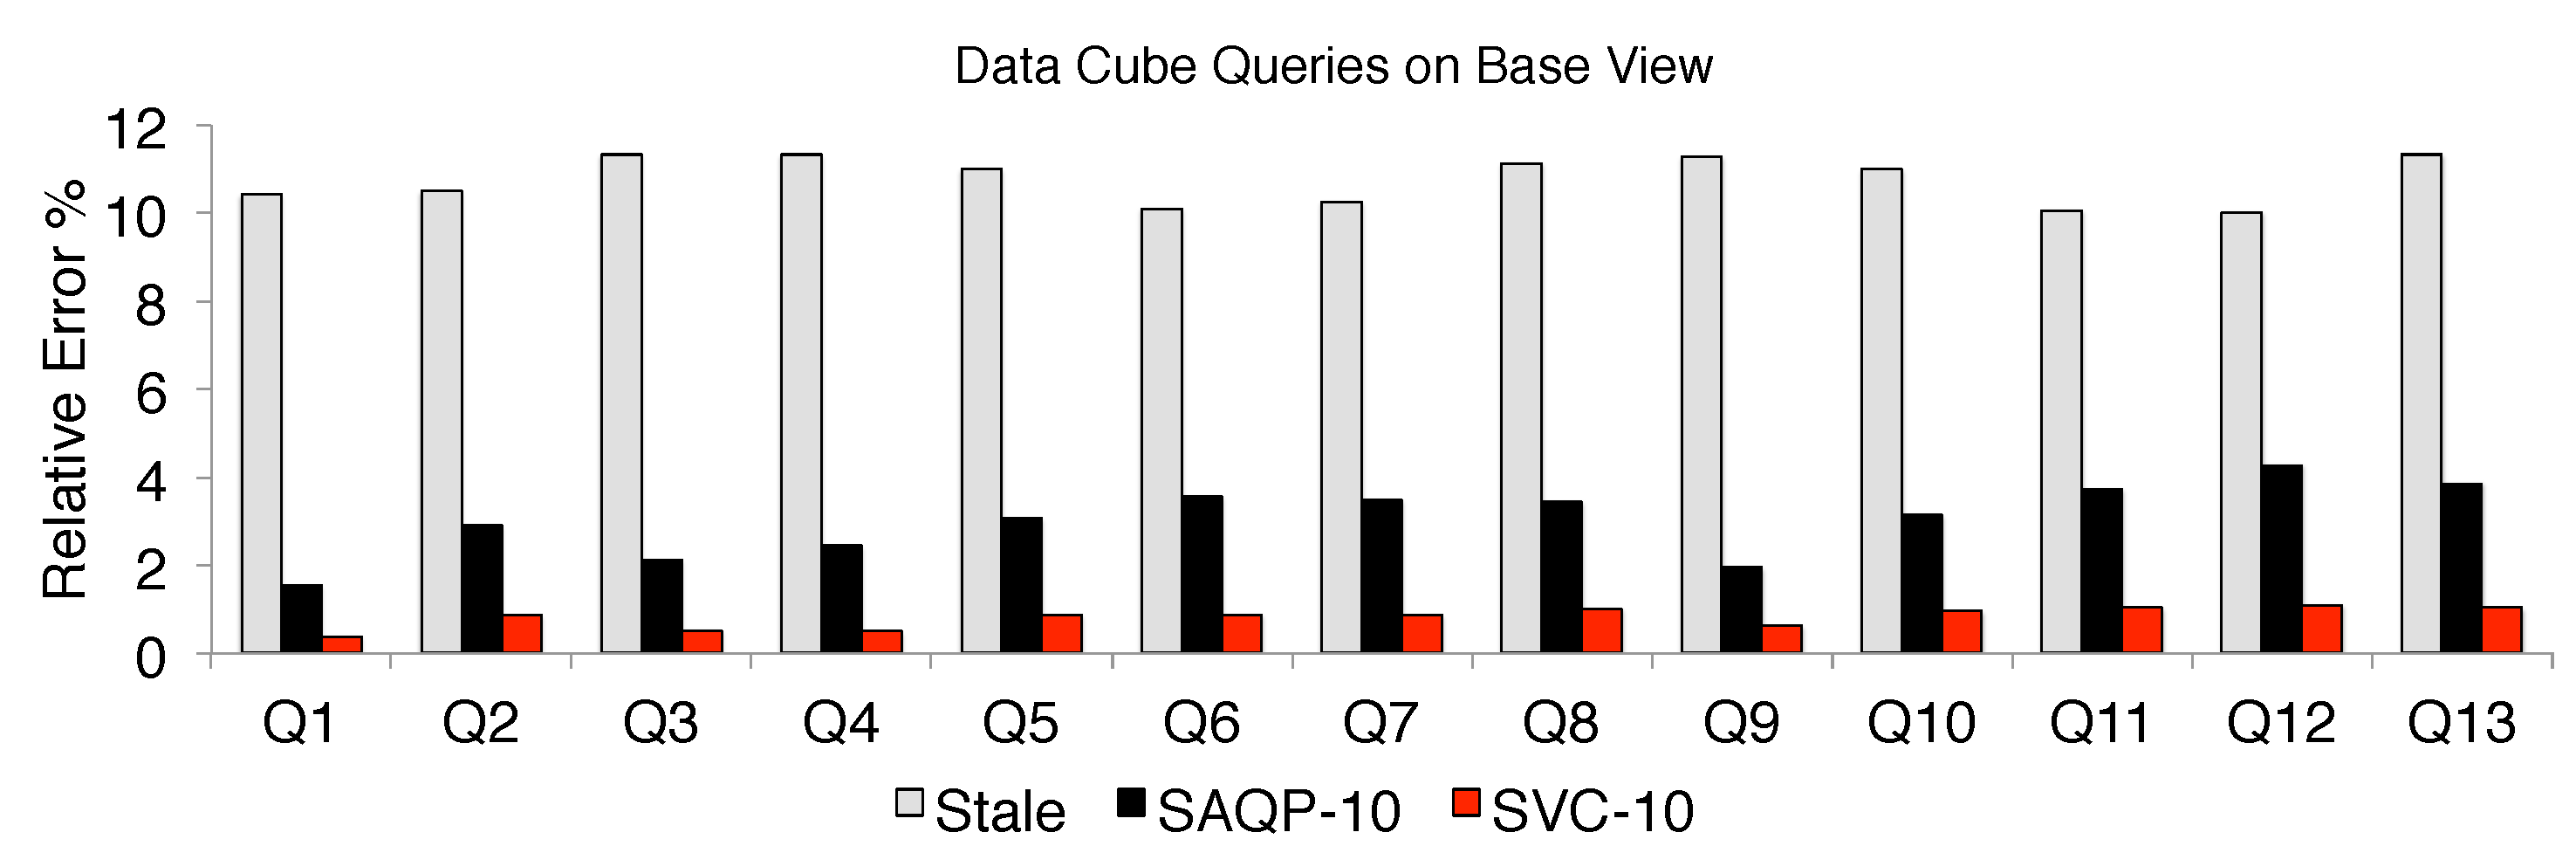
\includegraphics[scale=0.17]{exp/msdc_3.pdf}
   \caption{(a) In the aggregate view case, sampling can save significant maintenance time. (b) As the update size grows SVC tends towards an ideal speedup of 10x.\label{exp2-acc-sample}}
\end{figure}


\begin{figure}[t]
\centering
 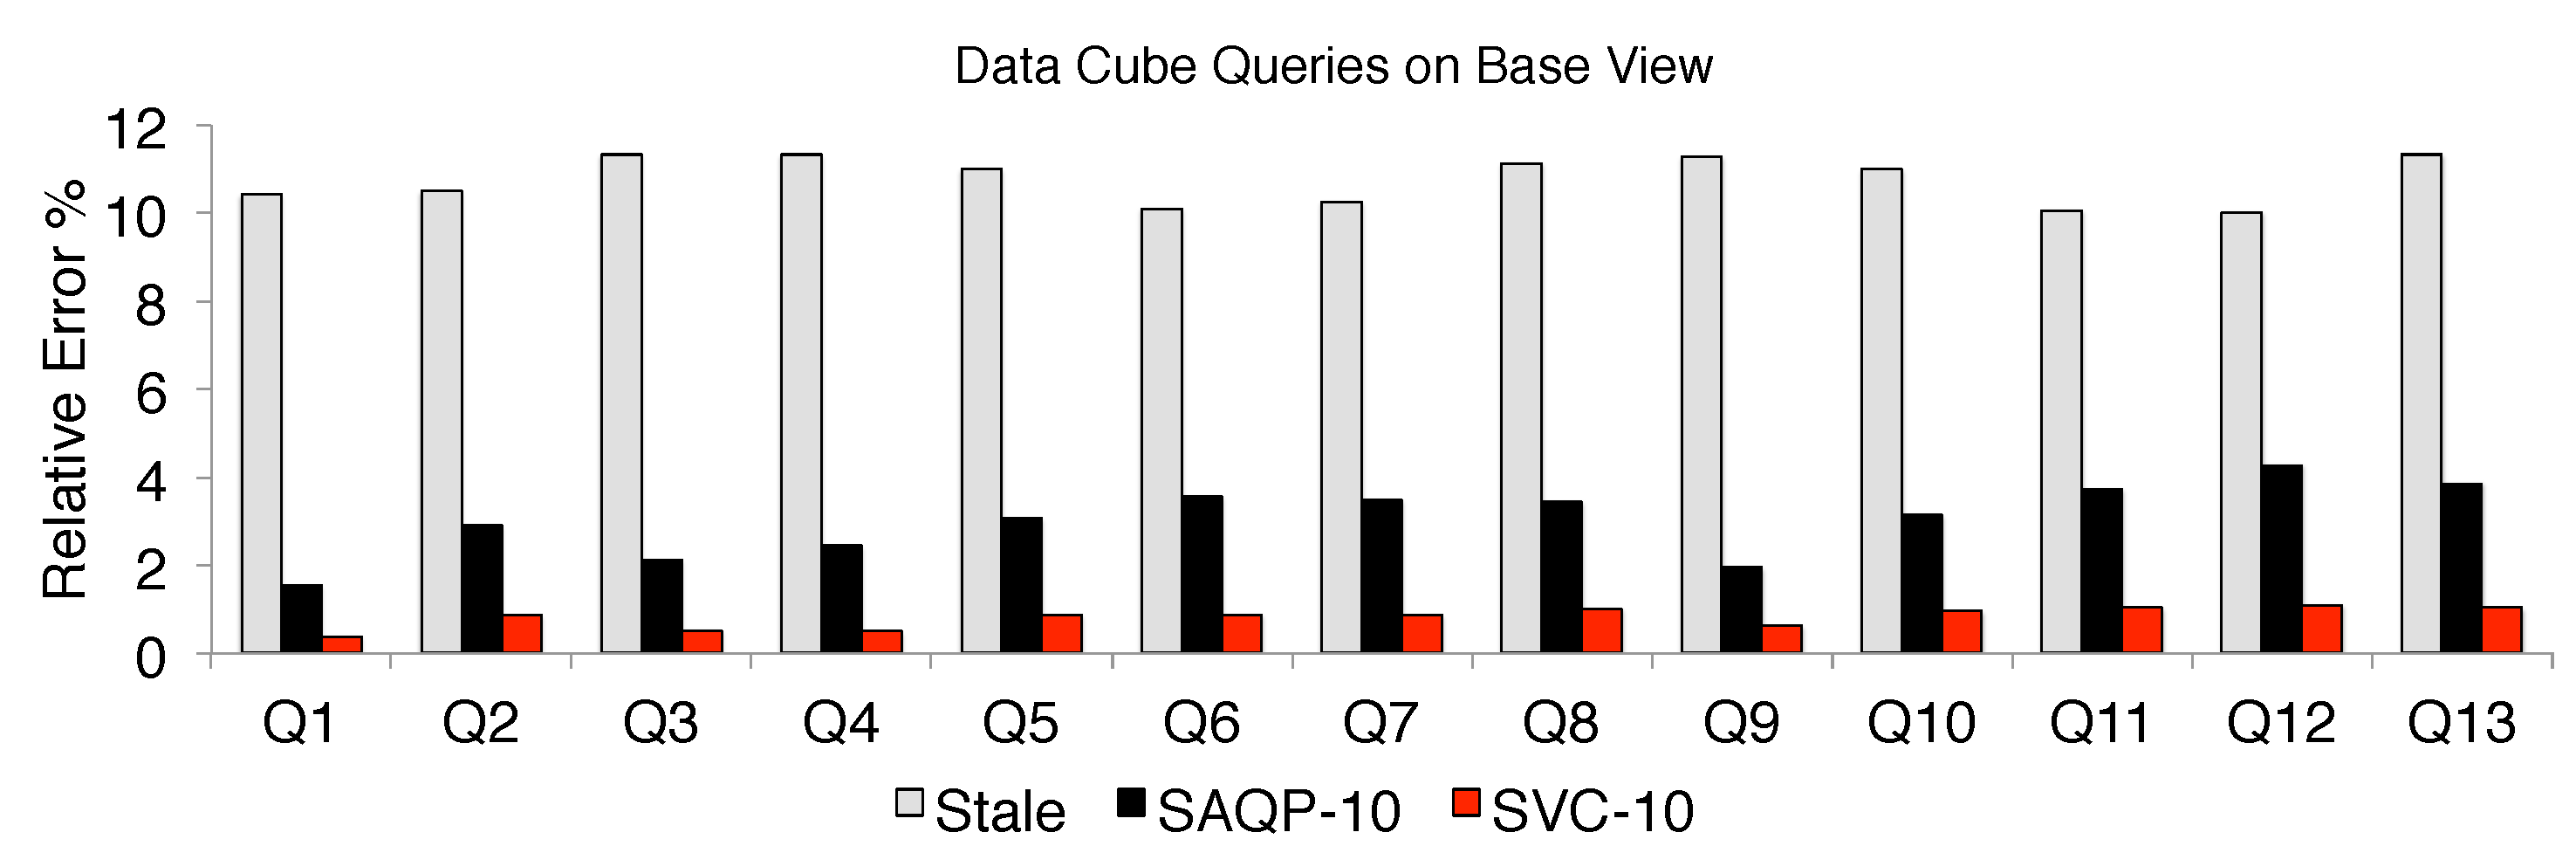
\includegraphics[scale=0.17]{exp/msdc_3.pdf}
   \caption{We measure the accuracy of each of the roll-up aggregate queries on this view. For a 10\% sample size and 10\% update size, we find that SVC+Corr is more accurate than SVC+AQP and No Maintenance.\label{exp2-acc-sample2}}
\end{figure}



\begin{figure}[t]
\centering
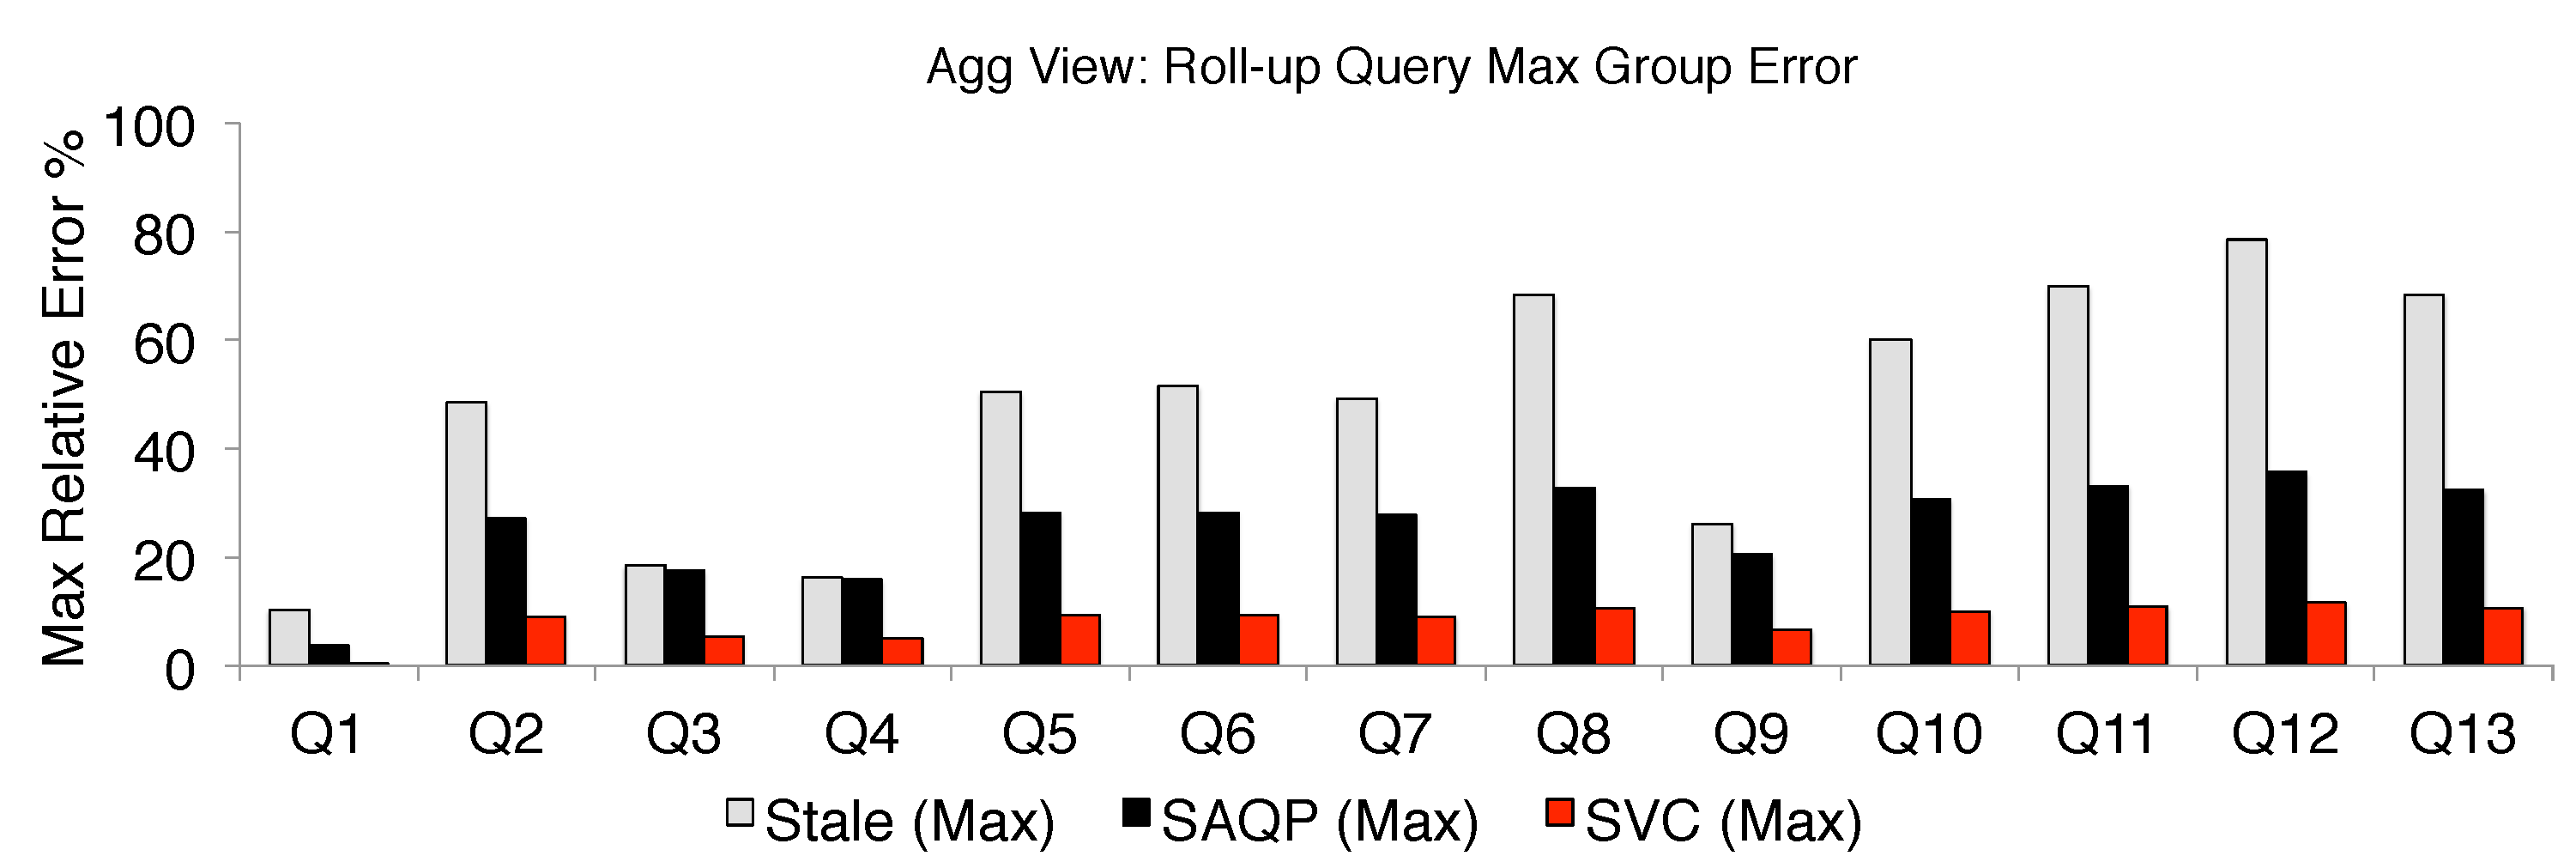
\includegraphics[scale=0.17]{exp/msdc_4.pdf}
   \caption{For 1GB of updates, we plot the max error as opposed to the median error in the previous experiments. Even though updates are 10\% of the dataset size, some queries are nearly 80\% incorrect. SVC helps significantly mitigate this error. \label{exp2-max}}
\end{figure}

\begin{figure}[t]
\centering
  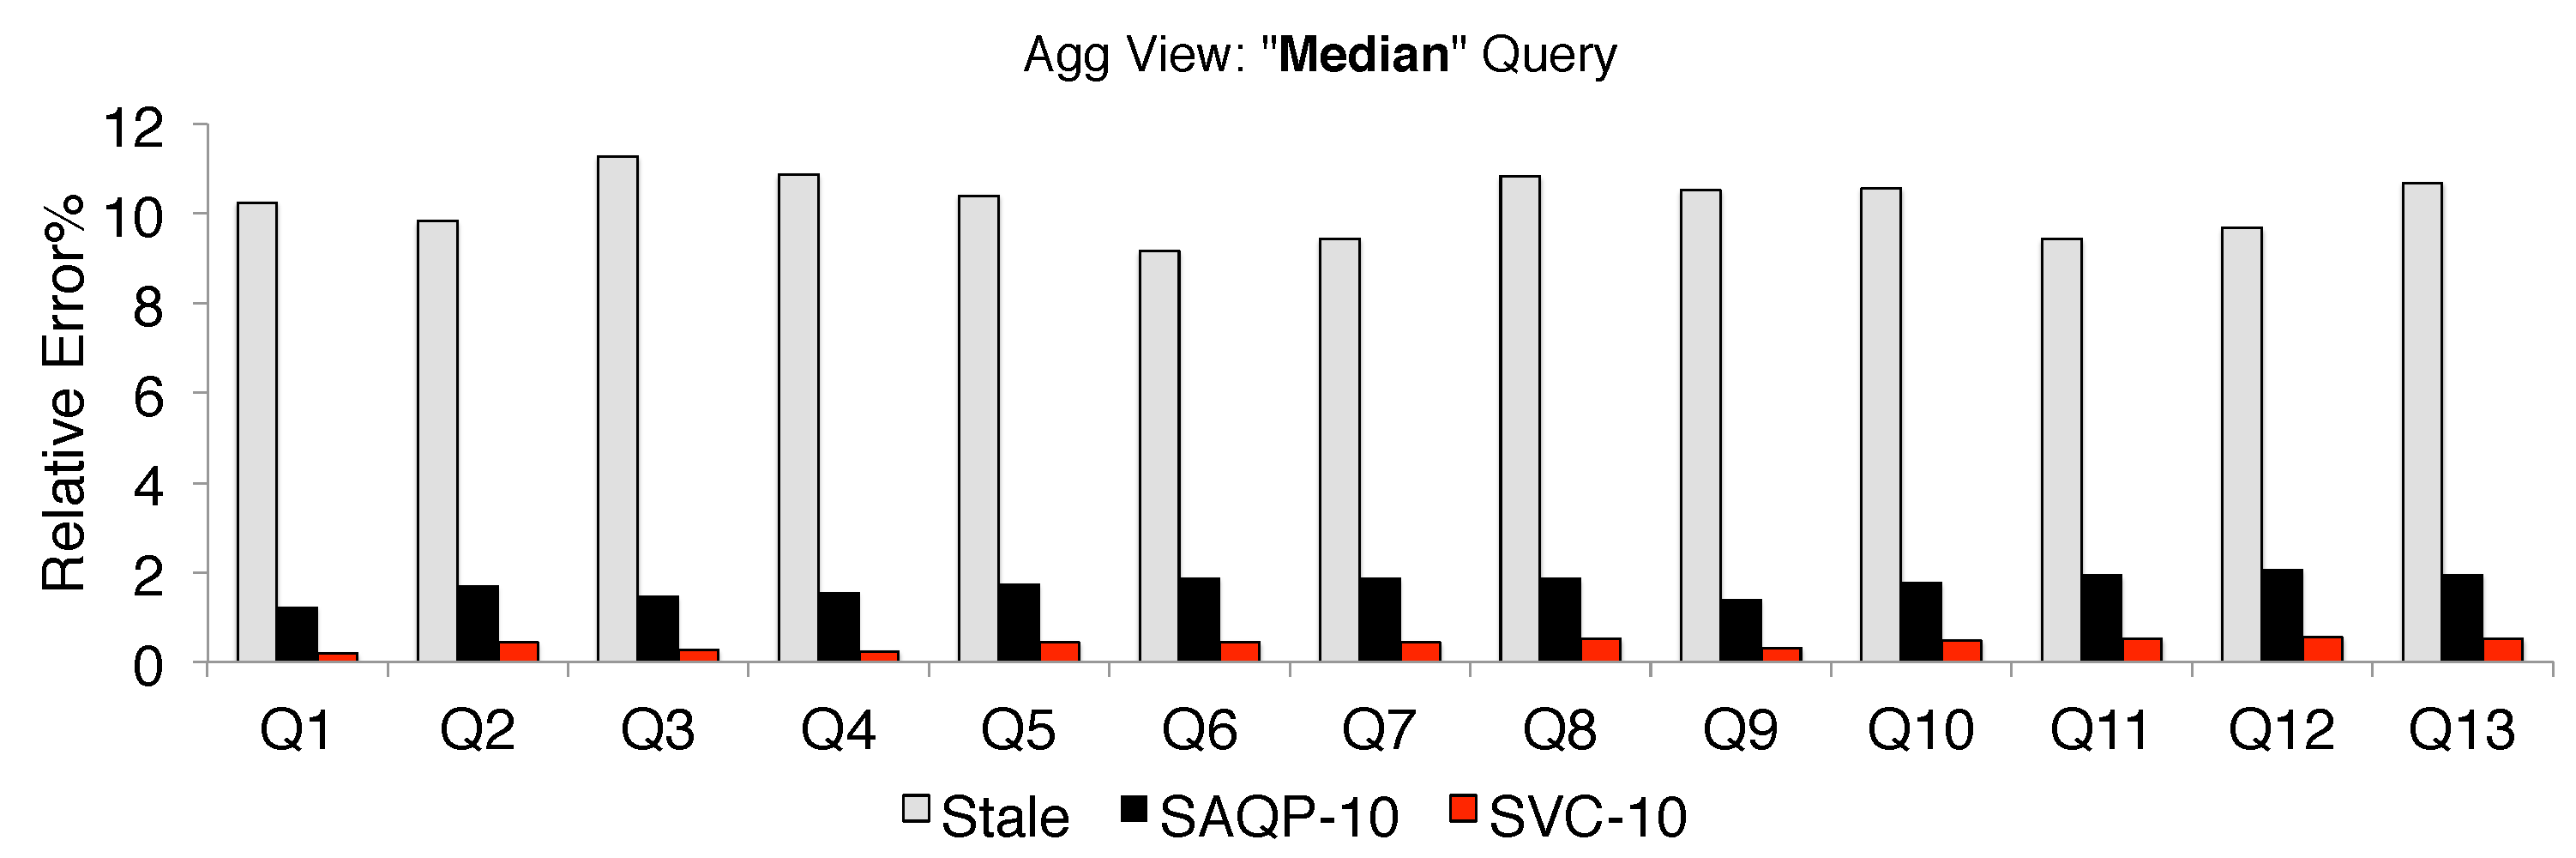
\includegraphics[scale=0.17]{exp/msdc_5.pdf}
  %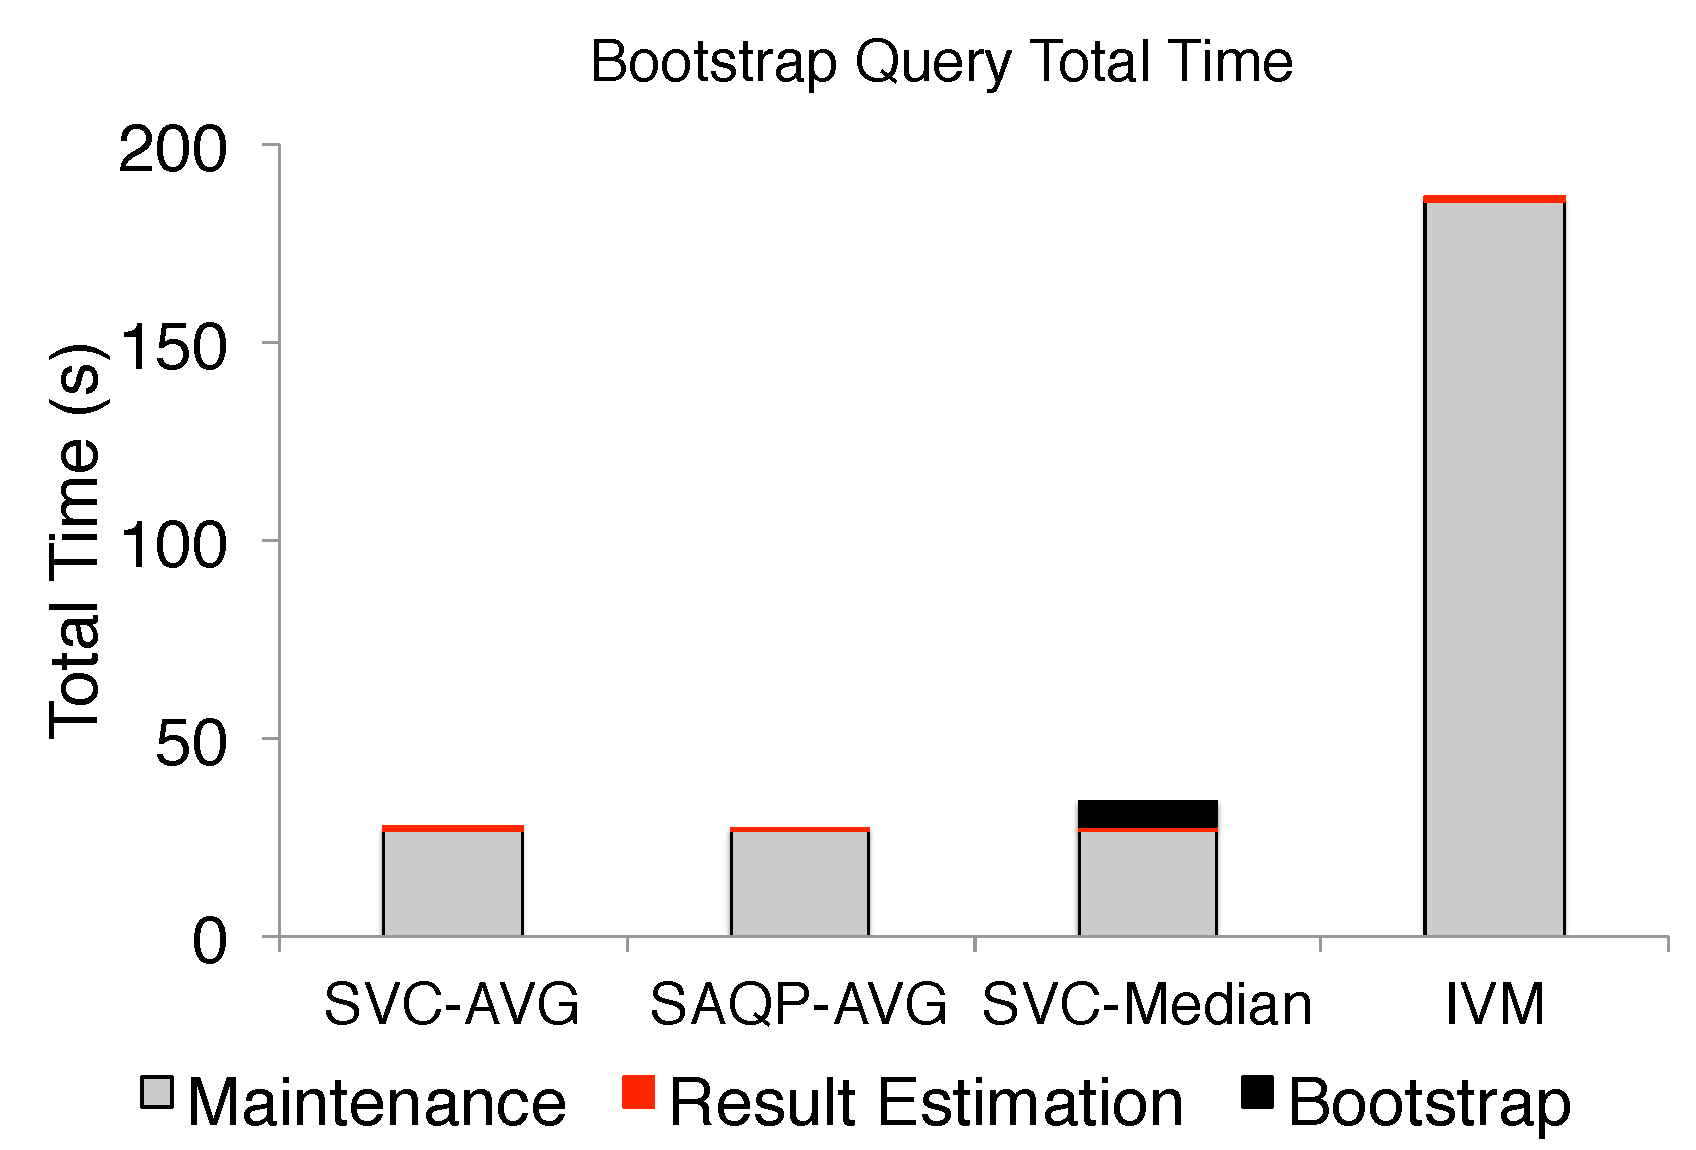
\includegraphics[scale=0.20]{exp/msdc_6.pdf}
 \caption{We run the same experiment but replace the \sumfunc query with a median query. We find that similarly SVC is more accurate.\label{exp2-median} }
\end{figure}

In our next experiment, we evaluate an aggregate view use case similar to a data cube.
We generate a 10GB base TPCD dataset with skew $z=1$, and derive the base cube as a materialized view from this dataset.
We add 1GB of updates and apply SVC to estimate the results of all of the ``roll-up" dimensions.

\textbf{Performance: }
We observed the same trade-off as the previous experiment where sampling significantly reduces the maintenance time (Figure \ref{exp2-acc-sample}(a)).
It takes 186 seconds to maintain the entire view, but a 10\% sample can be maintained in 26 seconds.
As before, we fix the sample size at 10\% and vary the update size.
We similarly observe that SVC becomes more efficient as the update size grows (Figure \ref{exp2-acc-sample}(b)), and at an update size of 20\%  the speedup is 8.7x.

\textbf{Accuracy: }
In Figure \ref{exp2-acc-sample2}, we measure the accuracy of each of the ``roll-up" aggregate queries on this view.
That is, we take each dimension and aggregate over the dimension.
We fix the sample size at 10\% and the update size at 10\%.
On average SVC+Corr is 12.9x more accurate than the stale baseline and 3.6x more accurate than SVC+AQP (Figure \ref{exp2-acc-sample}(c)). 

Since the data cubing operation is primarily constructed by group-by aggregates, we can also measure the max error for each of the aggregates.
We see that while the median staleness is close to 10\%, for some queries some of the group aggregates have nearly 80\% error (Figure \ref{exp2-max}).
SVC greatly mitigates this error to less than 12\% for all queries.

\textbf{Other Queries: }
Finally, we also use the data cube to illustrate how SVC can support a broader range of queries outside of \sumfunc, \countfunc, and \avgfunc.
We change all of the roll-up queries to use the \textbf{median} function (Figure \ref{exp2-median}).
First, both SVC+Corr and SVC+AQP are more accurate as estimating the median than they were for estimating sums. 
This is because the median is less sensitive to variance in the data.

\subsubsection{Complex Views}

\begin{figure}[t]
\centering
 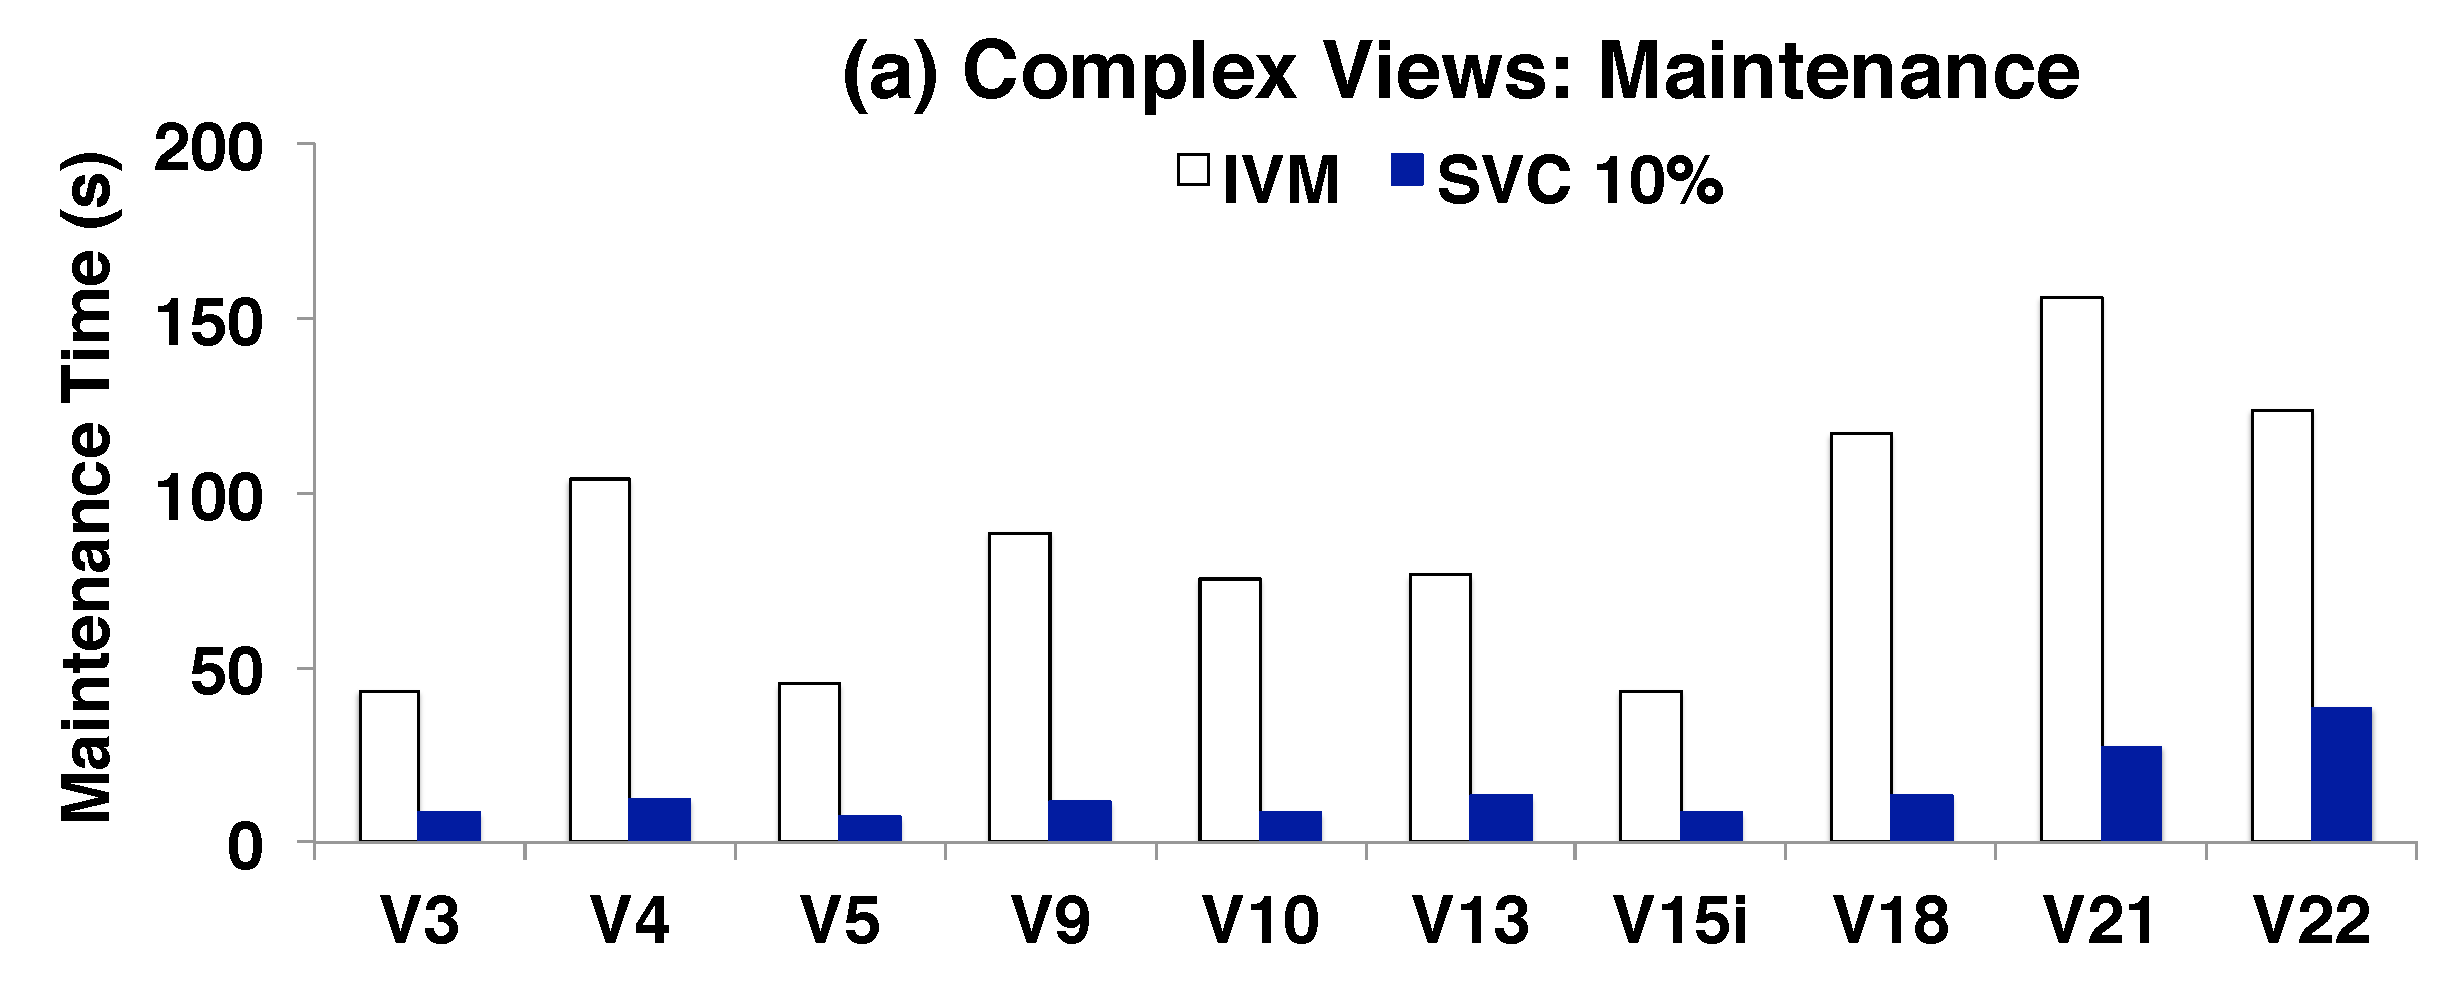
\includegraphics[scale=0.19]{exp/msqv_1.pdf}
 \caption{For 1GB update size, we compare maintenance time and accuracy of SVC with a 10\% sample on different views. V21 and V22 do not benefit as much from SVC due to nested query structures. \label{exp3-acc}}
\end{figure}

\begin{figure}[t]
\centering
 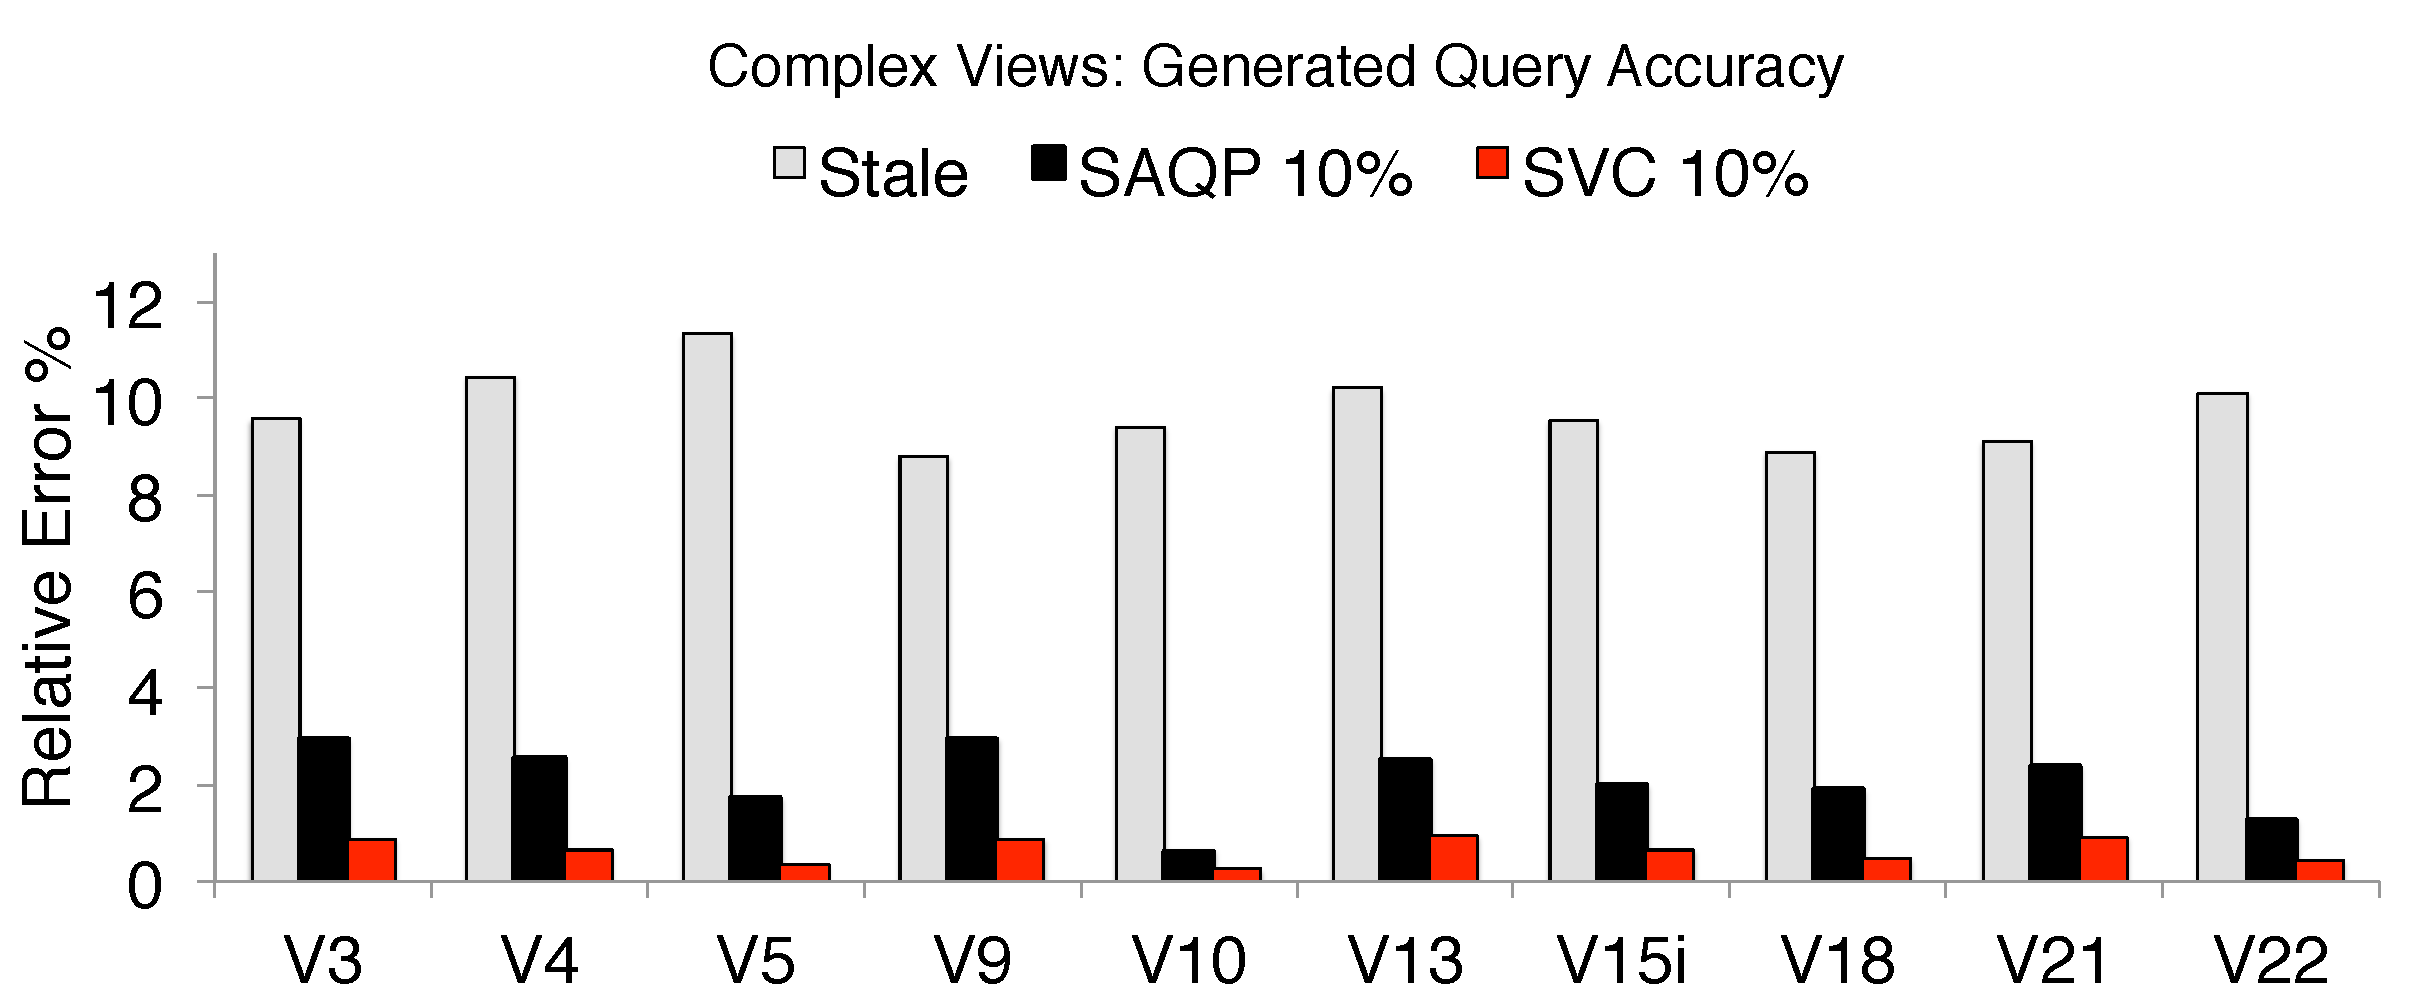
\includegraphics[scale=0.19]{exp/msqv_2.pdf}
 \caption{As before for a 10\% sample size and 10\% update size, SVC+Corr is more accurate than SVC+AQP and No Maintenance. \label{exp3-acc}}
\end{figure}

In the the last single-node experiment, we demonstrate the breadth of views supported by SVC.
Each parameterized TPCD query is treated as a materialized view, and we use the \textsf{qgen} program 
to generate 10 instances for each query.
When we report results, we average over these 10 instances for each of the query types.

\textbf{Performance: }
Figure \ref{exp3-acc}, shows the maintenance time for a 10\% sample compared to the full view.
As before, we find that sampling saves a significant amount of maintenance time.
However, this experiment illustrates how the view definitions plays a role in the efficiency of our approach.
For the last two views, V21 and V22, we see that sampling does not lead to as large of speedup indicated in our previous experiments.  
This is because both of those views contain nested structures which block the pushdown of our sampling.
V21 contains a subquery in its predicate that does not involve the primary key, but still requires a scan of the base relation to evaluate.
V22 contains a string transformation of a key blocking the push down.
There might be a way to derive an equivalent expression with joins that could be sampled more efficiently, and we will explore this in future work.
For the most part, these results are consistent with our previous experiments showing that SVC is faster than IVM and more accurate than SVC+AQP and no maintenance.


\subsubsection{Outlier Indexing}

\begin{figure}[t]
\centering
 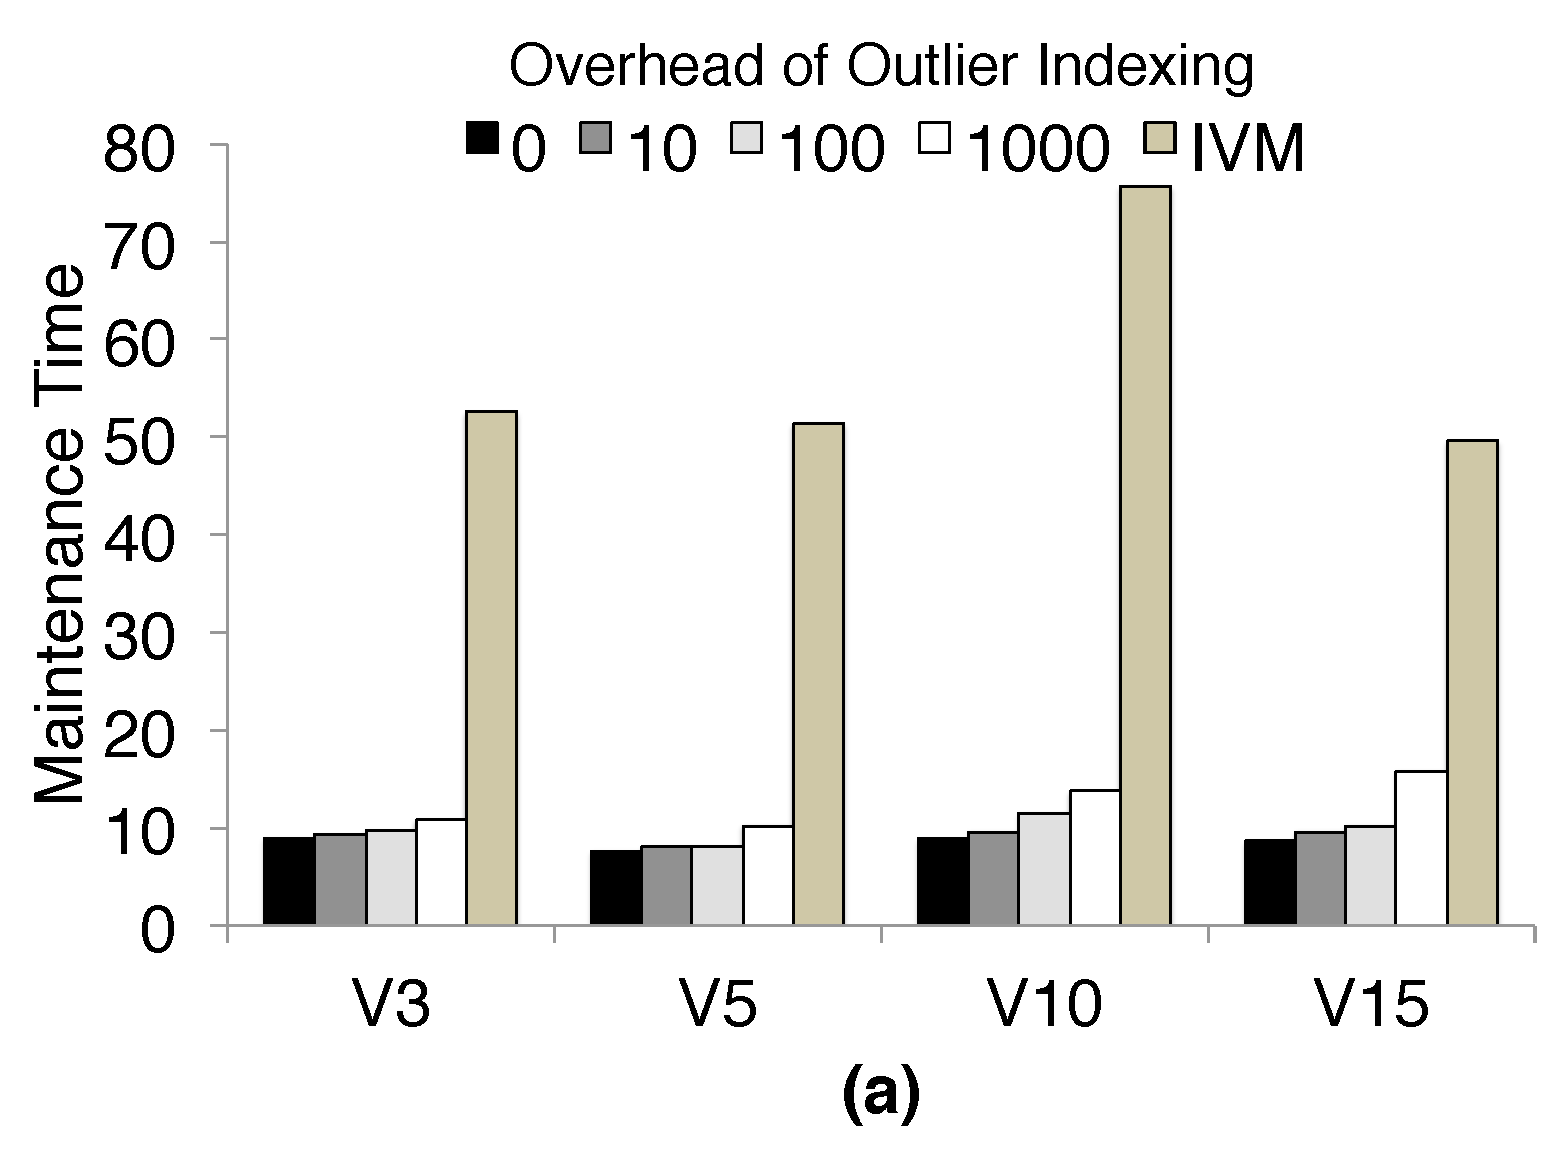
\includegraphics[scale=0.14]{exp/msoi_1.pdf}
 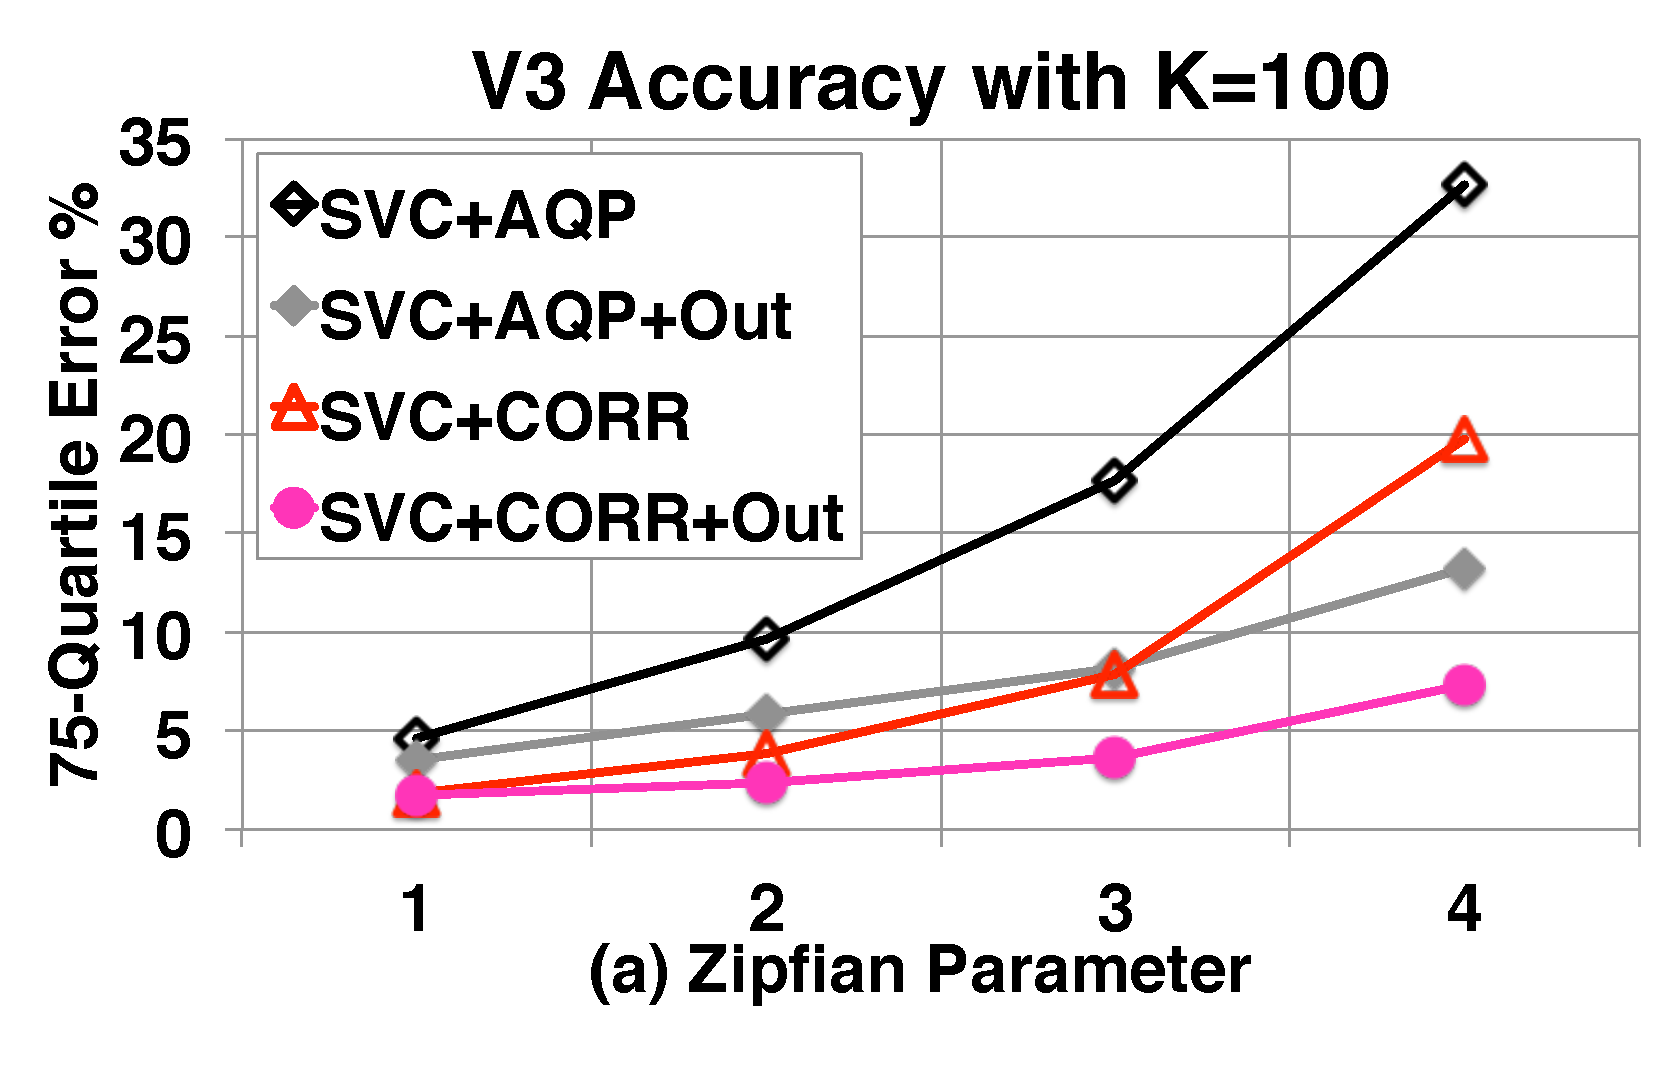
\includegraphics[scale=0.14]{exp/msoi_2.pdf}
 \caption{(a) For one view V3 and 1GB of updates, we plot the 75\% quartile error with different techniques as we vary the skewness of the data. We find that SVC with an outlier index of size 100 is the most accurate. (b) While the outlier index adds an overhead this is small relative to the total maintenance time. \label{exp5-oi}}
\end{figure}
We hinted at the sensitivity to dataset skew of sampling-based approaches earlier.
In our next experiment, we evaluate our outlier indexing.
Our outlier indices are constructed on the base relations.
We index the \textbf{l\_extendedprice} attribute in the \textbf{lineitem} table.
We evaluate the outlier index on the TPCD query views.

We find that four views: V3, V5, V10, V15, can benefit from this index with our push-up rules. 
These are four views dependent on \textbf{l\_extendedprice} that were also in the set of ``Complex" views chosen before.
We set an index of 100 records, and applied SVC+Corr and SVC+AQP to datasets with skew parameter $z=\{1,2,3,4\}$. 
We run the same queries as before, but this time we measure the error at the 75\% quartile.
In Figure \ref{exp5-oi}(a), we find in the most skewed dataset SVC with outlier indexing reduces query error by a factor of 2.
In the next Figure \big(Figure \ref{exp5-oi} (b)\big), we plot the overhead for outlier indexing for an index size of 0, 10, 100, and 1000.
While there is an overhead, it is still small compared to the gains made by sampling the maintenance strategy.

\subsection{Conviva}
In our next set of experiments, we applied SVC to a 1TB dataset of logs from Conviva.
We implement SVC on a 10-node Spark cluster. 

\subsubsection{Performance and Accuracy}
\begin{figure}[t]
\centering
 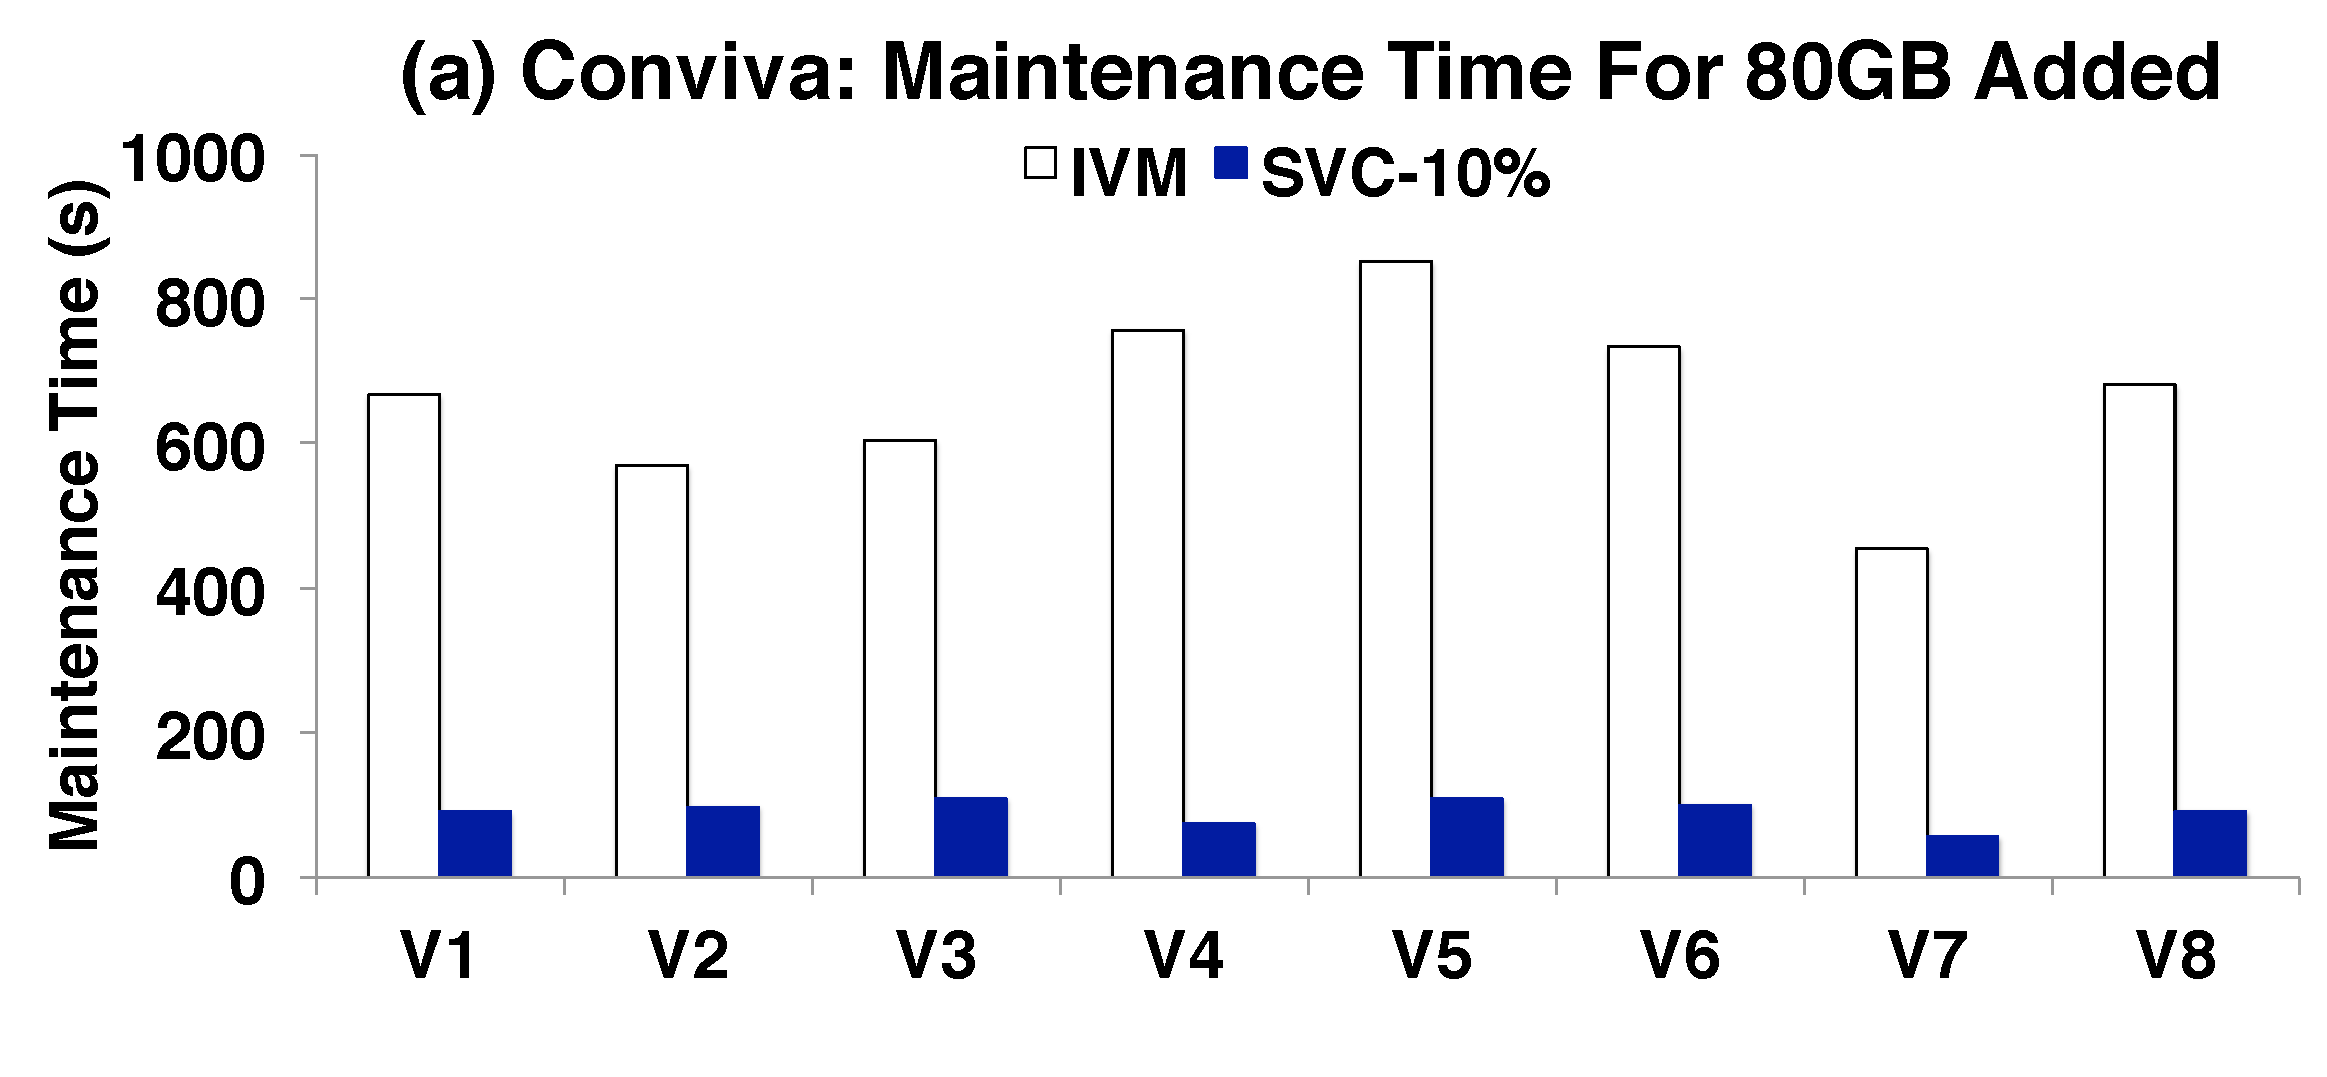
\includegraphics[scale=0.15]{exp/con_3.pdf}
 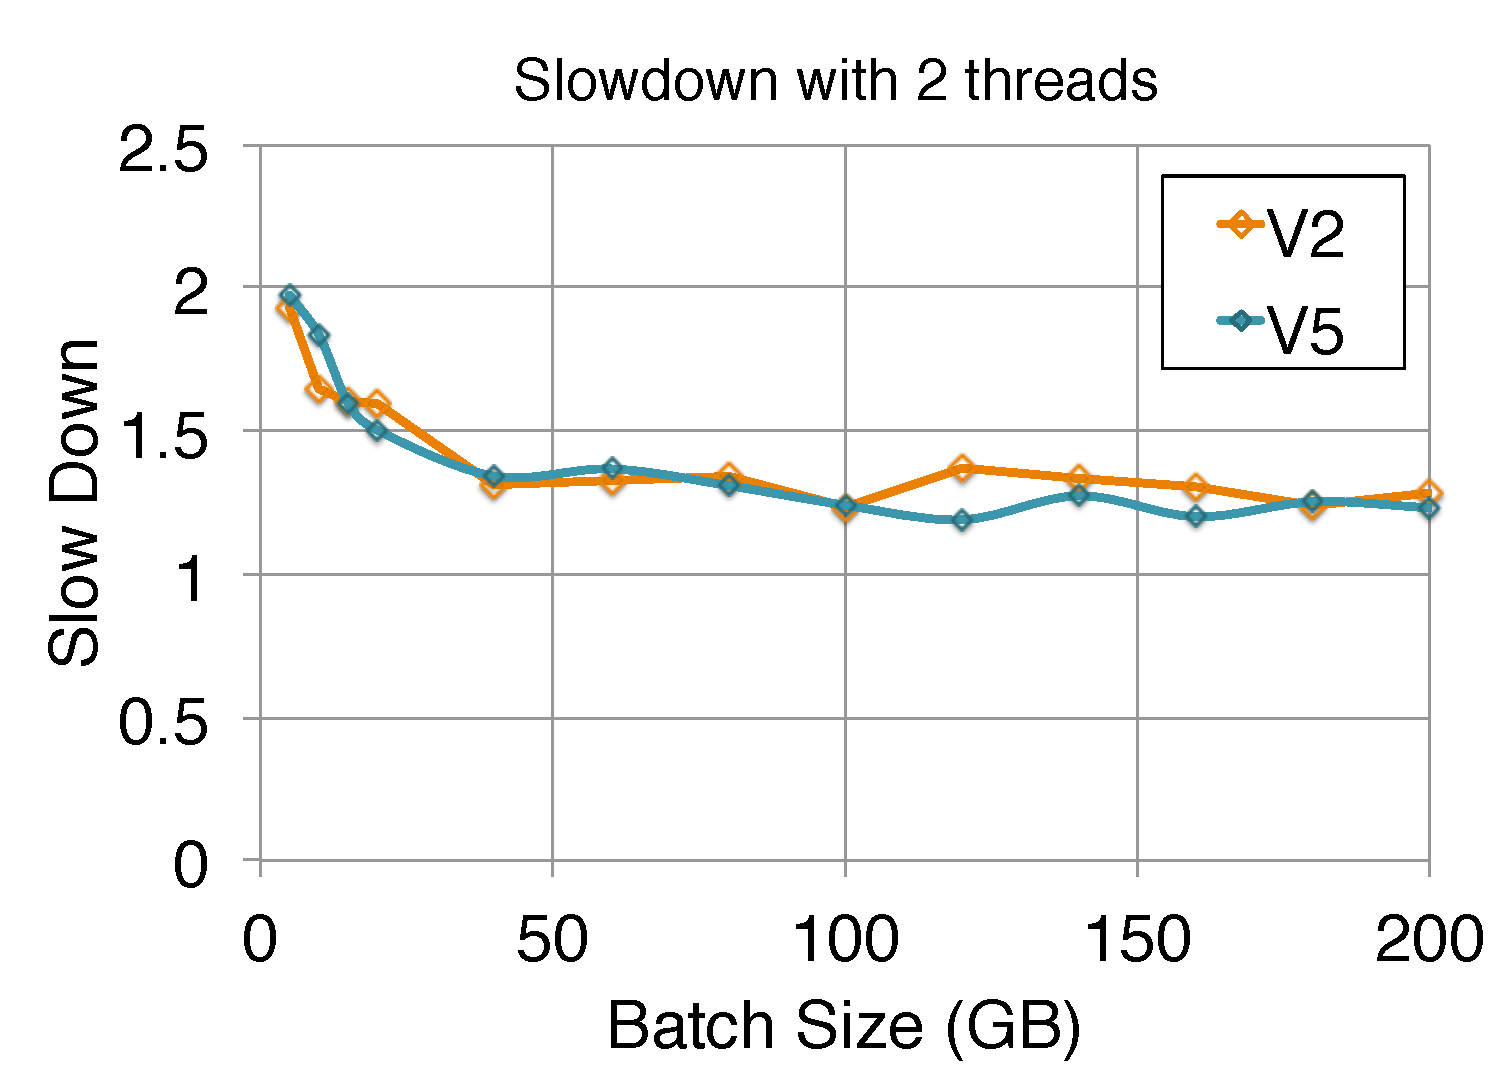
\includegraphics[scale=0.15]{exp/con_4.pdf}
 \caption{(a) We compare the maintenance time of SVC with a 10\% sample and full incremental maintenance, and find that as with TPCD SVC saves significant maintenance time. (b) We also compare SVC+Corr to SVC+AQP and No Maintenance and find it is more accurate. \label{conv-1}}
\end{figure}
We derive these views from 800GB of base data and add 80GB of updates.
In Figure \ref{conv-1}a, we show that while full maintenance takes nearly 800 seconds for one of the views, a 10\% sample SVC can complete sample maintenance in less than 100s for all of them.
On average SVC gives a 7.5x speedup.

SVC also gives highly accurate results with an average error of 0.98\%.
In the following experiments, we will use V2 and V5 as exemplary views.
V5 is the most expensive to maintain due to its nested query and V2 is a single level group by aggregate.
These results show consistency with our results on the synthetic datasets.

\subsubsection{End-to-end integration with periodic maintenance}
\begin{figure}[t]
\centering
 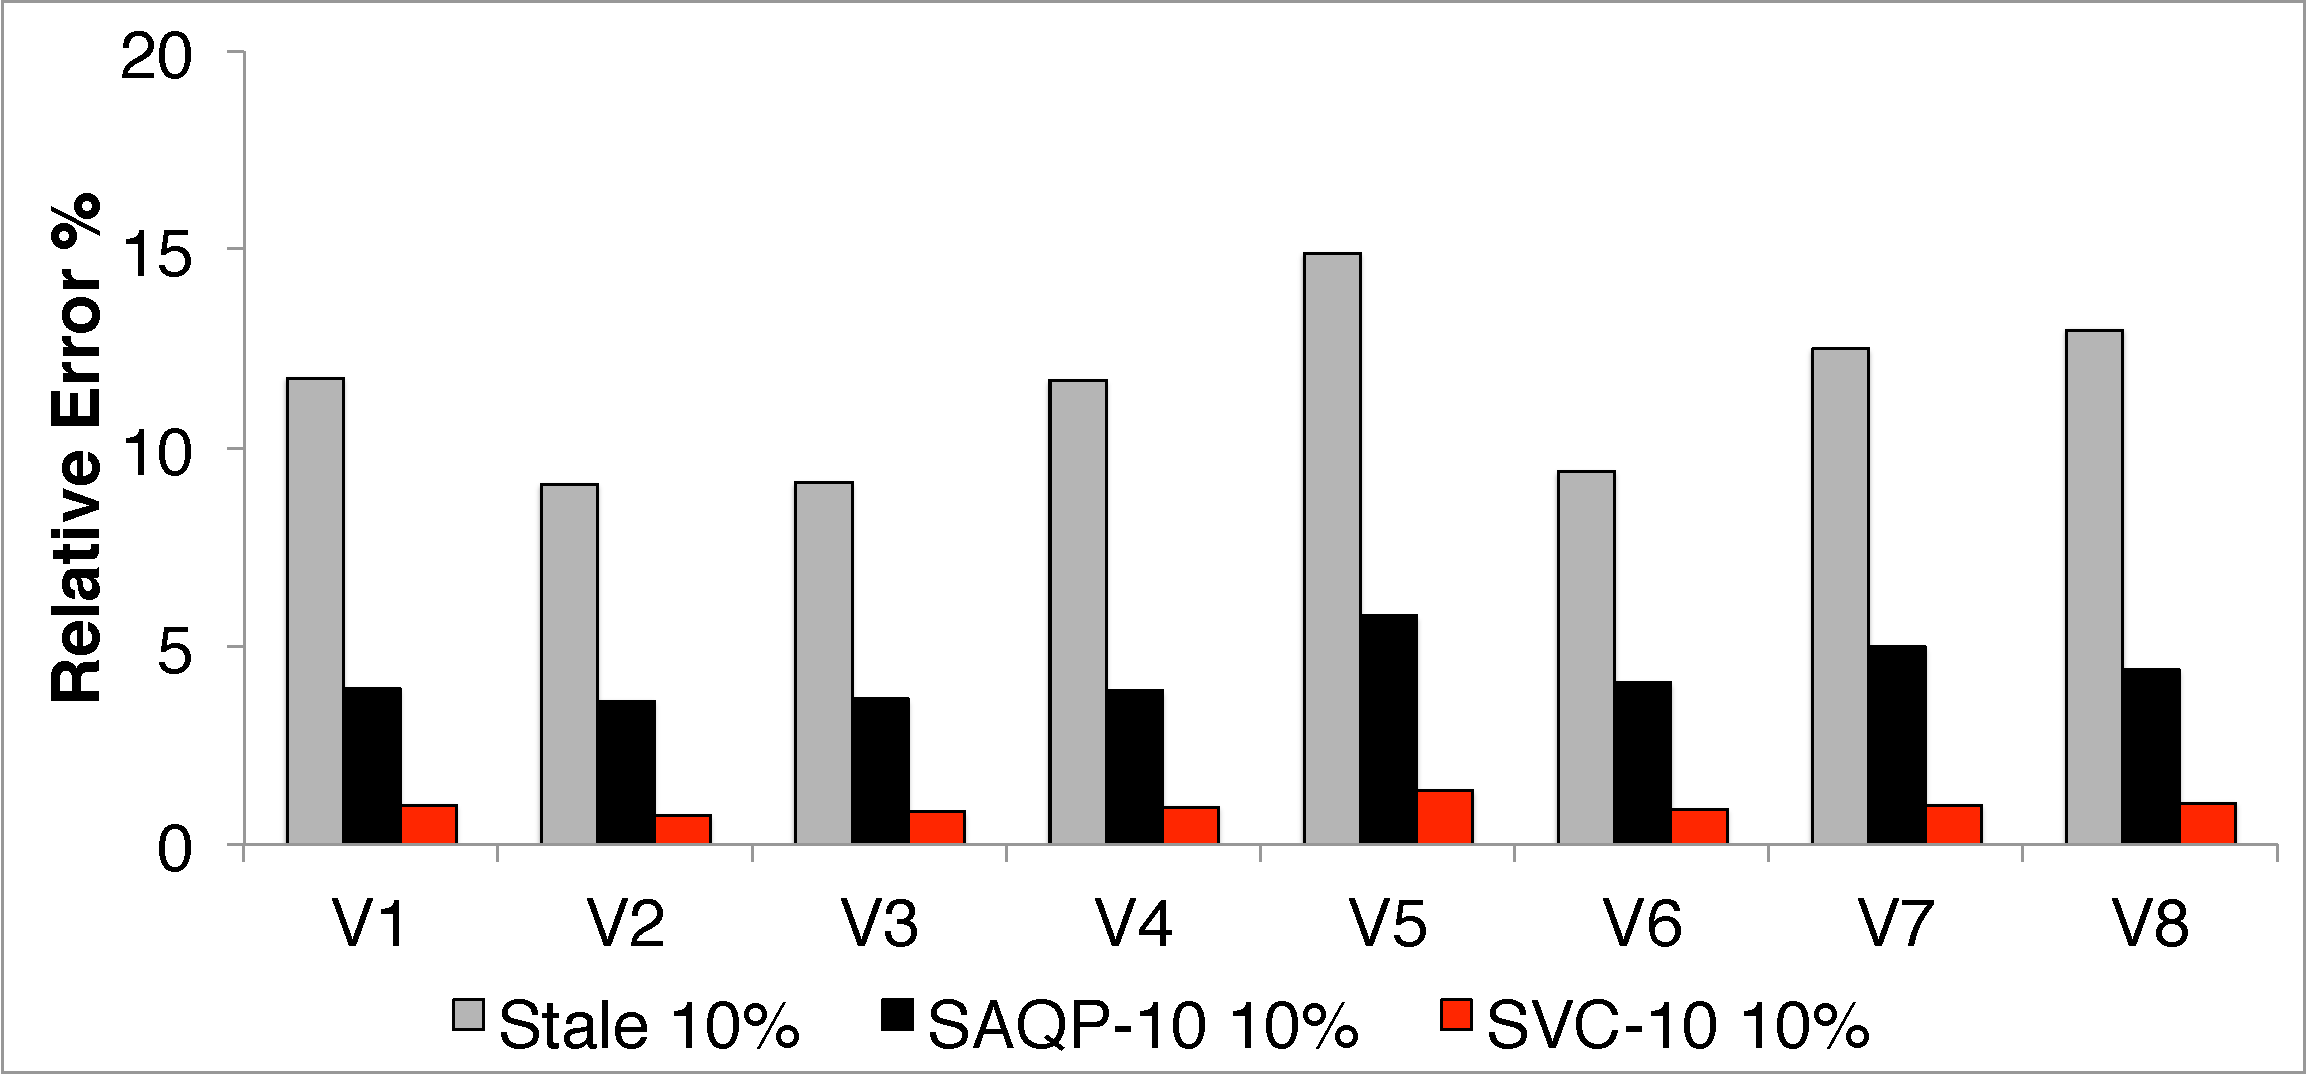
\includegraphics[scale=0.14]{exp/con_1.pdf}
 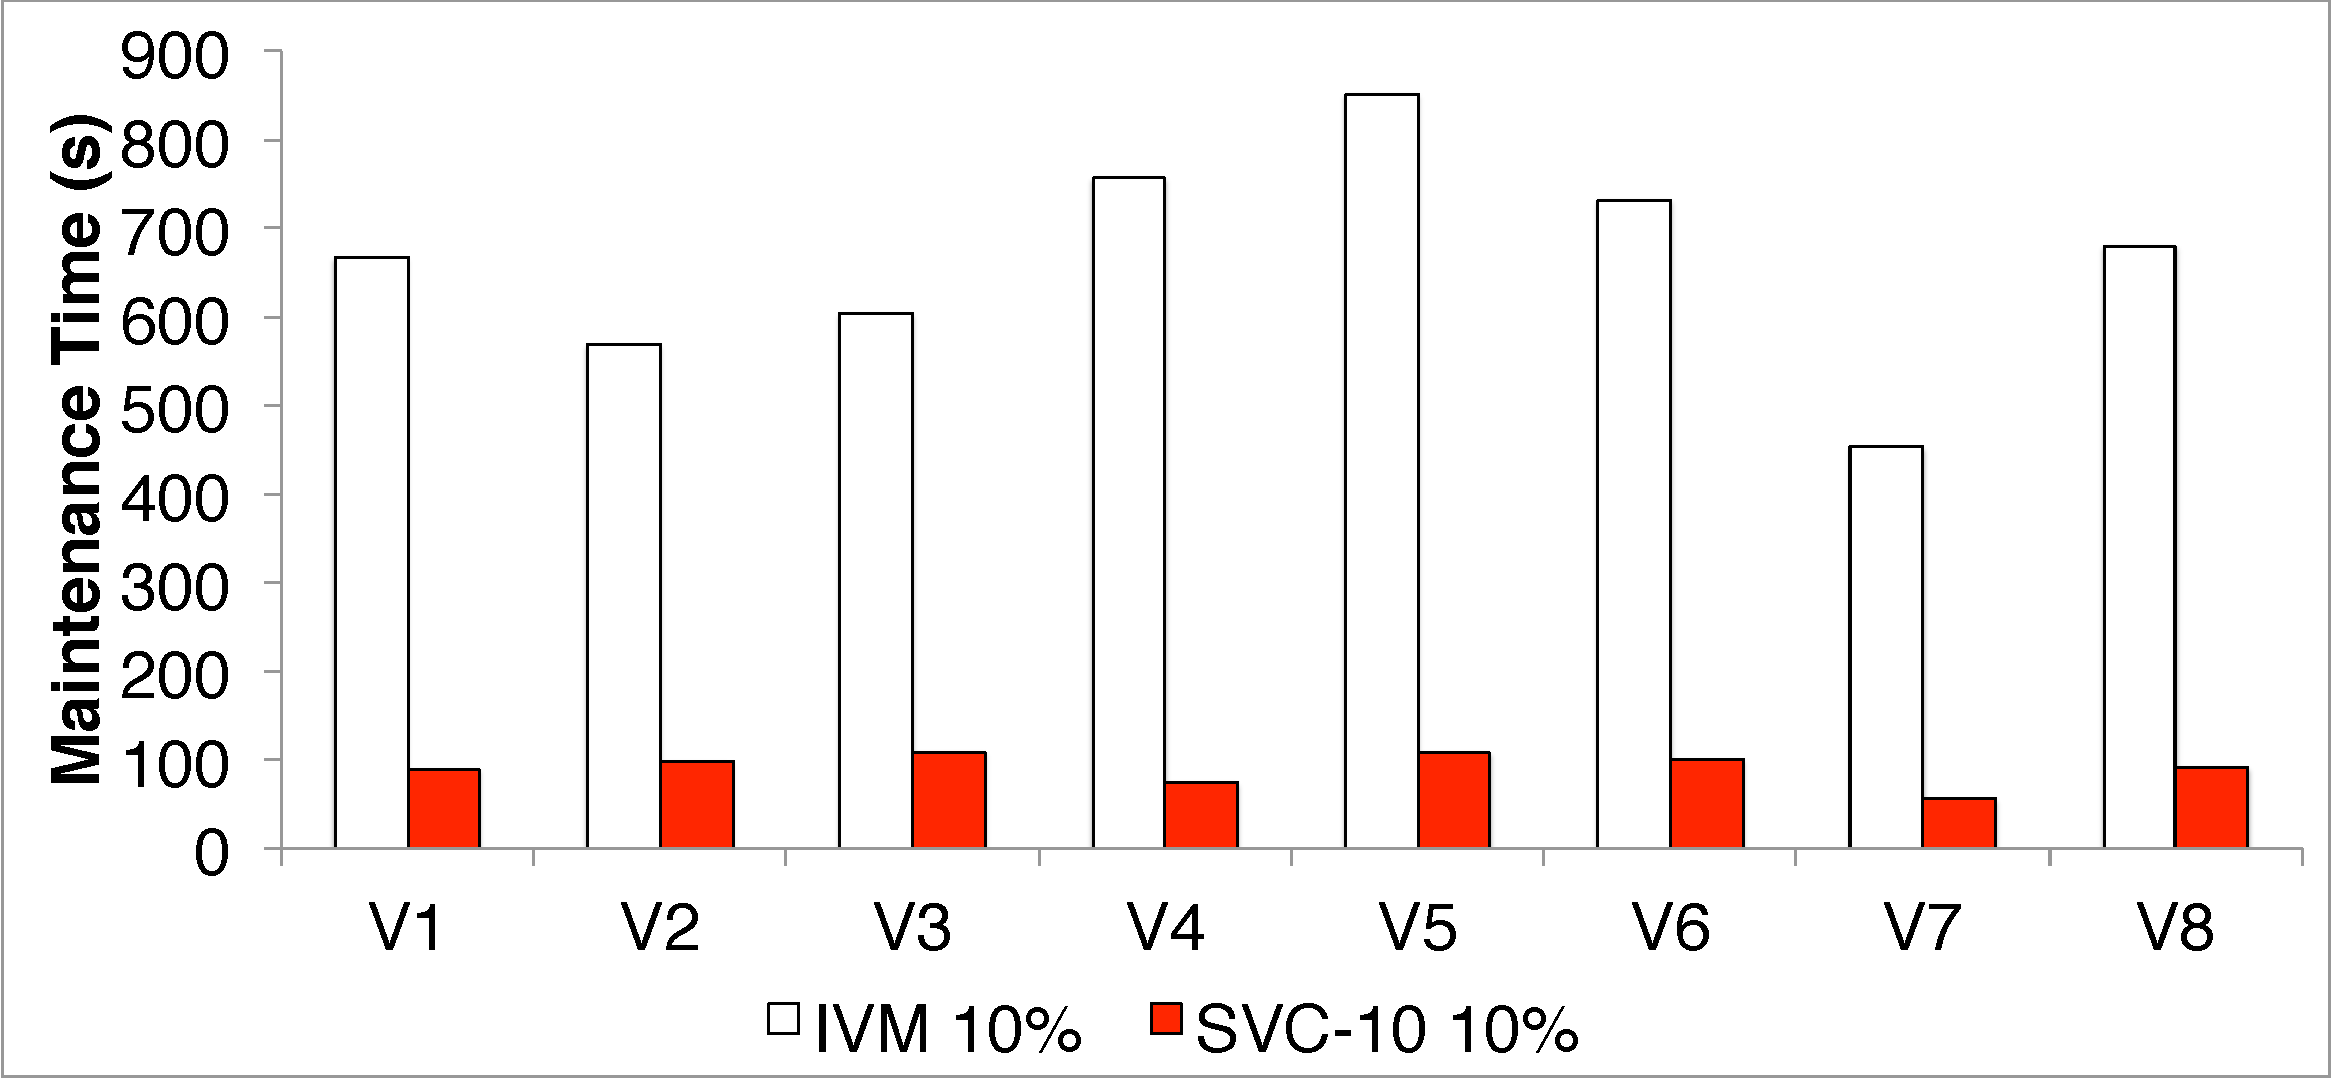
\includegraphics[scale=0.14]{exp/con_2.pdf}
 \caption{(a) Spark RDDs are most efficient when updated in batches. As batch sizes increase the system throughput increases. (b) When running multiple threads, the throughput reduces. However, larger batches are less affected by this reduction. \label{conv-2}}
\end{figure}

We devised an end-to-end experiment simulating a real integration with periodic maintenance.
However, unlike the MySQL case, Apache Spark does not support selective updates and insertions as the ``views" are immutable.
A further point is that the immutability of these views and Spark's fault-tolerance requires that the ``views" are maintained synchronously.
Thus, to avoid these significant overheads, we have to update these views in batches.
Spark does have a streaming variant \cite{zaharia2012discretized}, however, this does not support the complex SQL derived materialized views used in this paper, and still relies on mini-batch updates.

SVC and IVM will run in separate threads each with their own RDD materialized view.
In this application, both SVC and IVM maintain respective their RDDs with batch updates.
In this model, there are a lot of different parameters: batch size for periodic maintenance, batch size for SVC, sampling ratio for SVC, and the fact that concurrent threads may reduce overall throughput.
Our goal is to fix the throughput of the cluster, and then measure whether SVC+IVM or IVM alone leads to more accurate query answers.

\textbf{Batch sizes:} In Spark, larger batch sizes amortize overheads better.
In Figure \ref{conv-2}(a), we show a trade-off between batch size and throughput of Spark for V2 and V5.
Throughputs for small batches are nearly 10x smaller than the throughputs for the larger batches. 

\textbf{Concurrent SVC and IVM:} Next, we measure the reduction in throughput when running multiple threads.
We run SVC-10 in loop in one thread and IVM in another.
We measure the reduction in throughput for the cluster from the previous batch size experiment.
In Figure \ref{conv-2}(b), we plot the throughput against batch size when two maintenance threads are running.
While for small batch sizes the throughput of the cluster is reduced by nearly a factor of 2, for larger sizes the reduction is
smaller.
As we found in later experiments (Figure \ref{conv-5}), larger batch sizes are more amenable to parallel computation since there was more idle CPU time.

\textbf{Choosing a Batch Size:}
The results in Figure \ref{conv-2}(a) and Figure \ref{conv-2}(b) show that larger batch sizes are more efficient, however, larger batch sizes also lead to more staleness.
Combining the results in Figure \ref{conv-2}(a) and Figure \ref{conv-2}(b), for both SVC+IVM and IVM, we get cluster throughput as a function of batch size.
For a fixed throughput, we want to find the smallest batch size that achieves that throughput for both.
For V2, we fixed this at 700,000 records/sec and for V5 this was 500,000 records/sec.
For IVM alone the smallest batch size that met this throughput demand was 40GB for both V2 and V5.
And for SVC+IVM, the smallest batch size was 80GB for V2 and 100GB for V5. 
When running periodic maintenance alone view updates can be more frequent, and when run in conjunction with SVC it is less frequent. 

We run both of these approaches in a continuous loop, SVC+IVM and IVM, and measure their maximal error during a maintenance period.
There is further a trade-off with the sampling ratio, larger samples give more accurate estimates however between SVC batches they go stale.
We quantify the error in these approaches with the max error; that is the maximum error in a maintenance period (Figure \ref{conv-4}).
These competing objective lead to an optimal sampling ratio of 3\% for V2 and 6\% for V5.
At this sampling point, we find that applying SVC gives results 2.8x more accurate for V2 and 2x more accurate for V5.

\begin{figure}[t]
\centering
 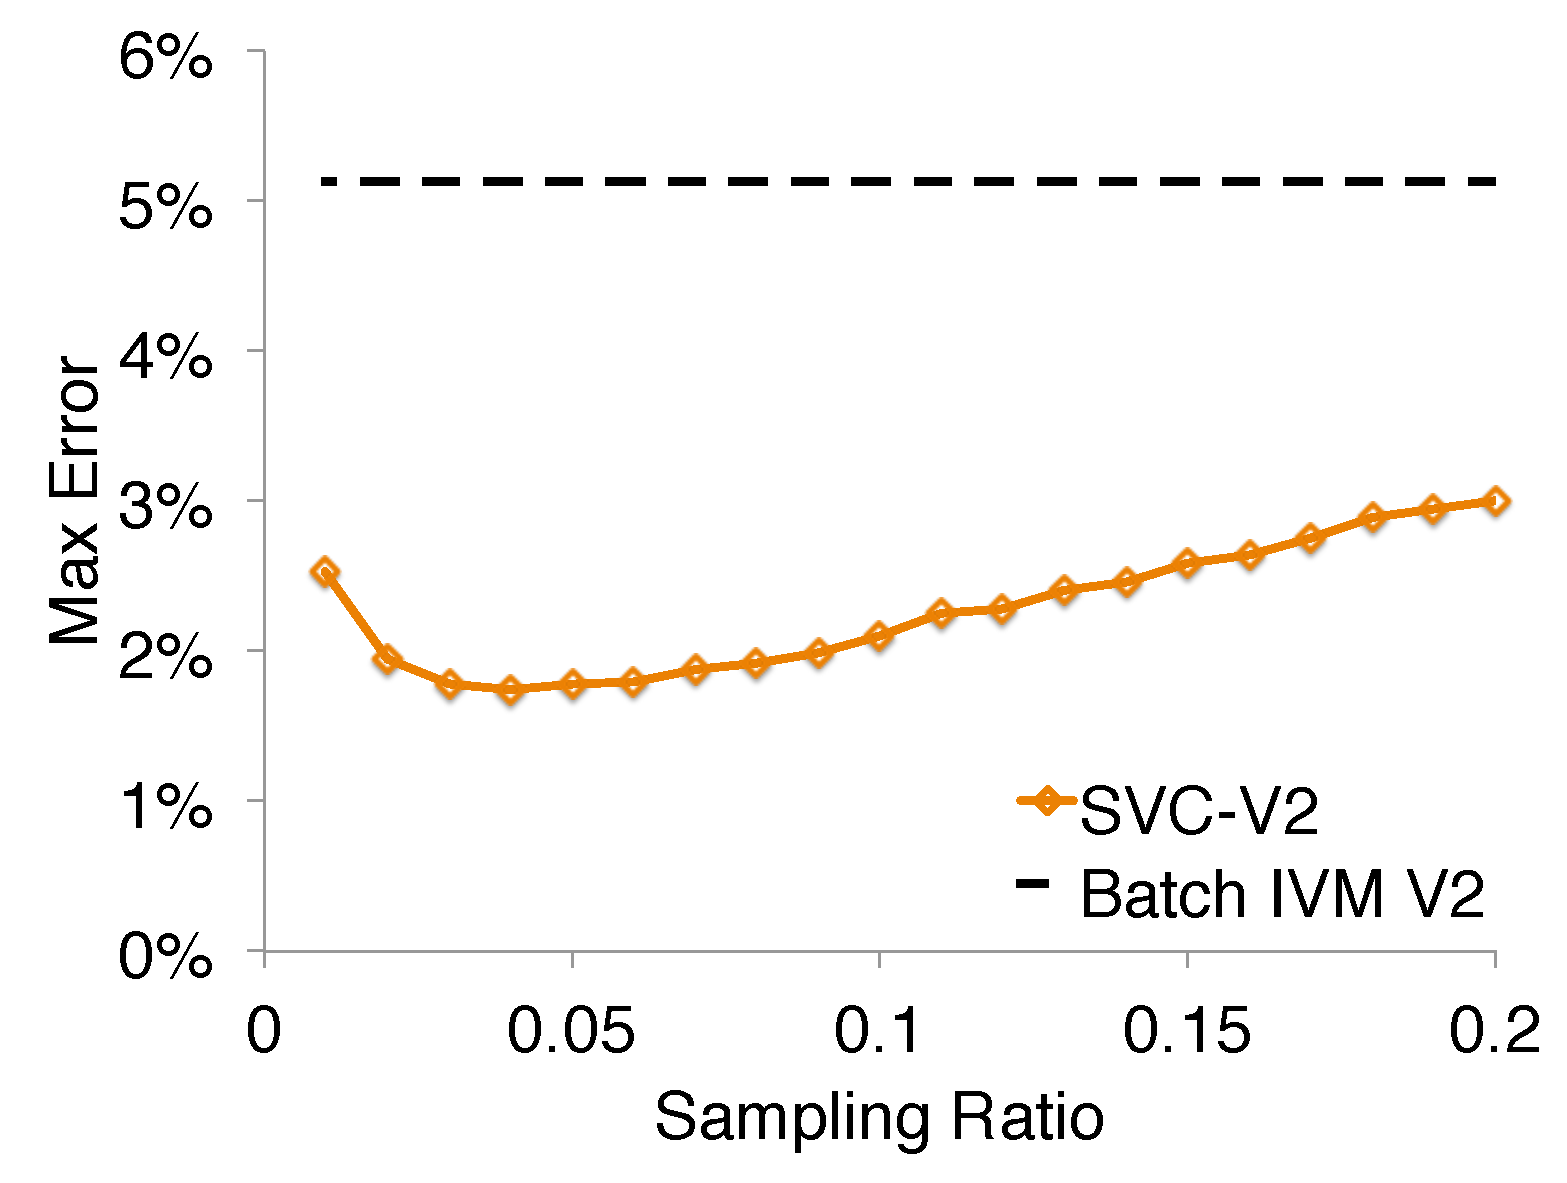
\includegraphics[scale=0.14]{exp/con_5.pdf}
 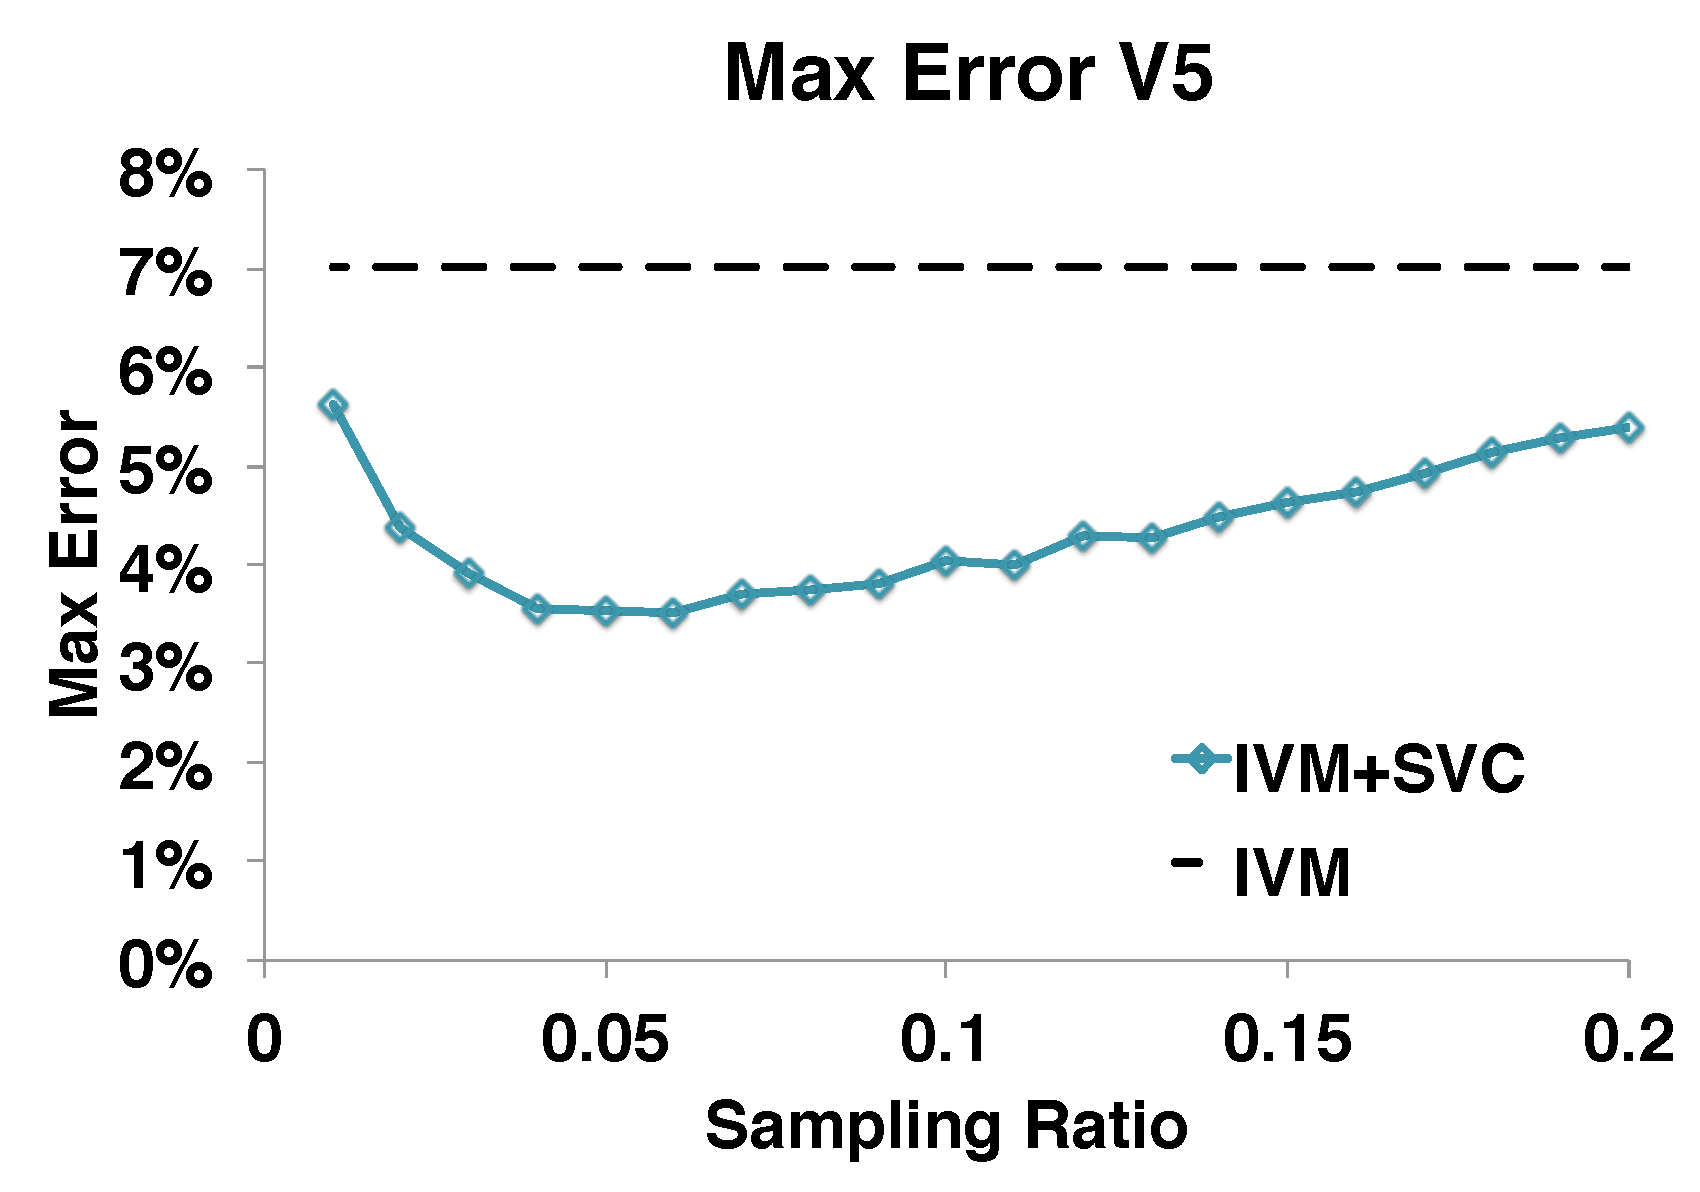
\includegraphics[scale=0.14]{exp/con_6.pdf}
 \caption{For a fixed throughput, SVC+Periodic Maintenance gives more accurate results for V2 and V5. \label{conv-4}} 
\end{figure}

\begin{figure}[t]
\centering
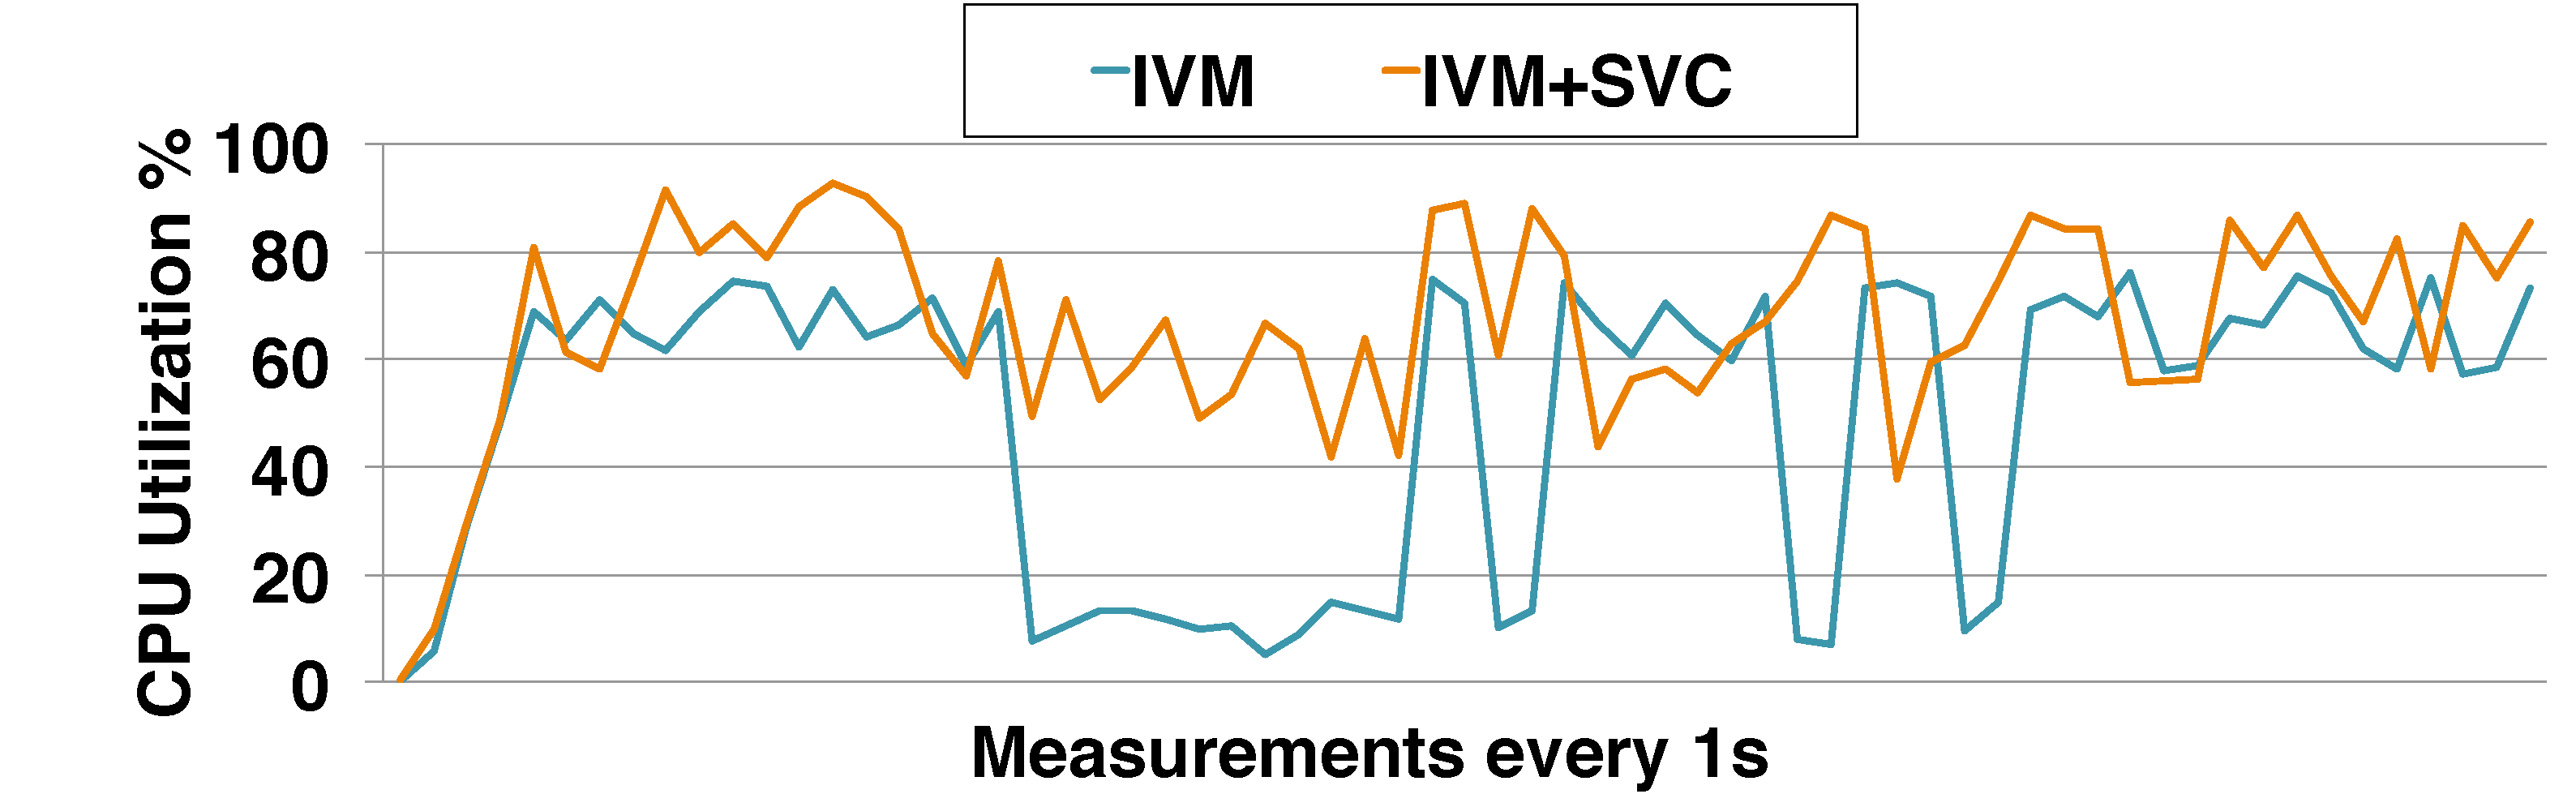
\includegraphics[scale=0.20]{exp/con_7.pdf}
 \caption{SVC better utilizes idle times in the cluster by maintaining the sample.\label{conv-5}} 
\end{figure}
To give some intuition on why SVC gives more accurate results, in Figure \ref{conv-5}, we plot the average CPU utilization of the cluster for both periodic IVM and SVC+periodic IVM. 
We find that SVC takes advantage of the idle times in the system; which are common during shuffle operations in a synchronous parallelism model.

In a way, these experiments present a worst-case application for SVC, yet it still gives improvements in terms of query accuracy.
In many typical deployments throughput demands are variable forcing maintenance periods to be longer, e.g., nightly.
The same way that SVC takes advantage of micro idle times during communication steps, it can provide large gains during controlled idle times when no maintenance is going on concurrently.


